\documentclass[sigplan,anonymous,review,nonacm]{acmart}

\usepackage{stmaryrd}
\usepackage{array}
\usepackage{mathtools}
\usepackage{tikz}
\usetikzlibrary{positioning,arrows.meta,calc,trees,matrix,fit,backgrounds,decorations.pathreplacing}
\usepackage{cancel}
\usepackage{forest}
\usepackage{xcolor}
\usepackage{fancyvrb}
\fvset{frame=single,framesep=3pt,fontsize=\small,xleftmargin=0pt,rulecolor=\color{black!25}}
\usepackage{subcaption}
\usepackage{xspace}
\newcount\draft \draft=0
\usepackage{xxx}
% Prose added during review, so a collaborator can see at a glance what is new.
% Goes black the moment \draft is 0.
\definecolor{newtext}{HTML}{1B7837}% green
\ifnum\draft=1
  \newcommand{\new}[1]{\textcolor{newtext}{#1}}
\else
  \newcommand{\new}[1]{#1}
\fi
\usepackage[capitalize,noabbrev]{cleveref}
\crefformat{section}{\S#2#1#3}
\Crefformat{section}{\S#2#1#3}
\crefformat{subsection}{\S#2#1#3}
\Crefformat{subsection}{\S#2#1#3}
\crefformat{subsubsection}{\S#2#1#3}
\Crefformat{subsubsection}{\S#2#1#3}
\crefmultiformat{section}{\S#2#1#3}{ and~\S#2#1#3}{, \S#2#1#3}{ and~\S#2#1#3}
\Crefmultiformat{section}{\S#2#1#3}{ and~\S#2#1#3}{, \S#2#1#3}{ and~\S#2#1#3}
\crefmultiformat{subsection}{\S#2#1#3}{ and~\S#2#1#3}{, \S#2#1#3}{ and~\S#2#1#3}
\Crefmultiformat{subsection}{\S#2#1#3}{ and~\S#2#1#3}{, \S#2#1#3}{ and~\S#2#1#3}
\crefrangeformat{section}{\S#3#1#4--\S#5#2#6}
\Crefrangeformat{section}{\S#3#1#4--\S#5#2#6}
\crefrangeformat{subsection}{\S#3#1#4--\S#5#2#6}
\Crefrangeformat{subsection}{\S#3#1#4--\S#5#2#6}
\crefrangeformat{subsubsection}{\S#3#1#4--\S#5#2#6}
\Crefrangeformat{subsubsection}{\S#3#1#4--\S#5#2#6}

\setlength{\emergencystretch}{3em}

\settopmatter{printfolios=true}

\newcommand{\push}{\ensuremath{\mathtt{push}}}
\newcommand{\pop}{\ensuremath{\mathtt{pop}}}
\newcommand{\flush}{\ensuremath{\mathtt{flush}}}
\newcommand{\csem}[1]{\mathcal{C}\llbracket #1 \rrbracket}
\newcommand{\psem}[1]{\mathcal{P}\llbracket #1 \rrbracket}
\newcommand{\eqR}{=_R}
% \notation: a notation name from the formal model. Math-italic, usable in
% both text and math mode, and does not swallow the space that follows it in
% text. Write \pol{}s for a plural, \pol{} before any other brace group.
\newcommand{\notation}[1]{\ensuremath{#1}\ifmmode\else\xspace\fi}
\newcommand{\pol}{\notation{\mathit{pol}}}
\newcommand{\pifo}{\notation{\mathit{pifo}}}
\newcommand{\zz}{\notation{\mathit{z}}}
\newcommand{\stt}{\notation{\mathit{state}}}
\newcommand{\pth}{\notation{\mathit{path}}}
\newcommand{\survivor}{\notation{\mathit{survivor}}}
\newcommand{\slotstates}{\notation{\mathit{slot\_states}}}
\newcommand{\nodestate}{\notation{\mathit{node\_state}}}
\newcommand{\arm}{\notation{\mathit{arm}}}
\newcommand{\disc}{\notation{D}}
\newcommand{\rio}{\textsf{Rio}}
\newcommand{\Strict}{\textsf{Strict}}
\newcommand{\Strictstar}{\textsf{Strict}^{*}}
\newcommand{\WFQ}{\textsf{WFQ}}
\newcommand{\RR}{\textsf{RoundRobin}}
\newcommand{\FIFO}{\textsf{FIFO}}
\newcommand{\Add}{\textsf{Add}}
% \dsetminus: a compressed double set-minus, for striking a flow set from a service map.
\newcommand{\dsetminus}{\mathbin{\smallsetminus\mkern-3mu\smallsetminus}}
\newcommand{\ChangeMeta}{\textsf{ChangeMeta}}
\newcommand{\Quiesce}{\textsf{Quiesce}}
\newcommand{\Remove}{\textsf{Remove}}
\newcommand{\Designate}{\textsf{Designate}}
\newcommand{\Undesignate}{\textsf{Undesignate}}
\newcommand{\Retire}{\textsf{Retire}}
\newcommand{\Replace}{\textsf{Replace}}

% Small drawn queues for the tree figures.
% \leafbox{k}: a 5-cell buffer whose rightmost k cells each hold a packet (a filled disc).
\newcommand{\leafbox}[1]{%
\begin{tikzpicture}[baseline=-0.55ex, x=2.0ex, y=2.0ex,
   cell/.style={draw=black!55, rounded corners=0.3ex, minimum size=1.9ex, inner sep=0pt, line width=0.45pt}]
  \foreach \i in {1,...,5}{%
    \ifnum\i>\numexpr5-#1\relax
      \node[cell, fill=black!8] at (\i,0) {};
      \fill[black!78] (\i,0) circle (0.42ex);
    \else
      \node[cell] at (\i,0) {};
    \fi}%
\end{tikzpicture}%
}
% \pifobox{list}: one rounded cell per comma-separated entry, left to right (popped right to left).
\newcommand{\pifobox}[1]{%
\begin{tikzpicture}[baseline=-0.55ex, x=2.15ex, y=2.0ex,
   cell/.style={draw=black!55, rounded corners=0.3ex, minimum size=1.9ex, inner sep=1pt, font=\scriptsize, line width=0.45pt}]
  \foreach \c [count=\i] in {#1}{%
    \node[cell] at (\i,0) {\(\c\)};}%
\end{tikzpicture}%
}
% House style for opaque subtrees: a colored triangle is a subtree; dots along its base
% are the packets buffered inside it. Colors are Okabe-Ito (colorblind-friendly).
\definecolor{oldcol}{HTML}{0072B2}% blue
\definecolor{newcol}{HTML}{E69F00}% orange
\newcommand{\subtri}[4]{% #1 color, #2 apex x, #3 apex y, #4 dot count (0-3)
  \draw[fill=#1!12, draw=#1, line width=0.6pt] (#2,#3) -- (#2-0.55,#3-0.9) -- (#2+0.55,#3-0.9) -- cycle;
  \ifcase#4\relax\or
    \fill[#1] (#2,#3-0.72) circle (1.3pt);\or
    \fill[#1] (#2-0.16,#3-0.72) circle (1.3pt); \fill[#1] (#2+0.16,#3-0.72) circle (1.3pt);\or
    \fill[#1] (#2-0.24,#3-0.72) circle (1.3pt); \fill[#1] (#2,#3-0.72) circle (1.3pt); \fill[#1] (#2+0.24,#3-0.72) circle (1.3pt);%
  \fi
}
% Freshly built material is shaded: \freshbehind{(a)(b)} lays the wash behind the named
% nodes. It sits on a background layer, so the wash can never ride over what it marks,
% and it is fitted to those nodes, so it can never drift off them either.
% anchor=center is load-bearing where a picture is drawn inside a \node, since such a
% picture inherits that node's anchor.
\pgfsetlayers{background,main}
\newcommand{\freshbehind}[1]{%
  \begin{pgfonlayer}{background}
    \node[fill=newcol!12, rounded corners=2pt, anchor=center, inner sep=3.5pt, fit=#1] {};
  \end{pgfonlayer}}
% Explicit-PIFO house style: leaf packets are colored dots by flavor (colored rounded box);
% internal index-PIFOs are gray with numbers; dropped entries get a steep red strikeout.
\definecolor{flowA}{HTML}{0072B2}% blue
\definecolor{flowB}{HTML}{E69F00}% orange
\definecolor{flowC}{HTML}{009E73}% green
\newcommand{\leafpifo}[2]{% #1 color, #2 packet count
\begin{tikzpicture}[baseline=-0.55ex, x=1.75ex, y=1.75ex]
  \draw[rounded corners=0.3ex, draw=#1, fill=#1!12, line width=0.7pt] (0.5,-0.62) rectangle ({#2+0.5},0.62);
  \foreach \i in {1,...,#2}{\fill[#1] (\i,0) circle (0.44ex);}%
\end{tikzpicture}%
}
\newcommand{\numpifo}[2]{% #1 entry list, #2 struck positions (0 for none)
\begin{tikzpicture}[baseline=-0.55ex, x=1.75ex, y=1.75ex]
  \foreach \e [count=\i] in {#1}{\xdef\lastn{\i}}%
  \draw[draw=black!60, fill=black!6, rounded corners=0.3ex, line width=0.6pt] (0.5,-0.62) rectangle ({\lastn+0.5},0.62);
  \foreach \e [count=\i] in {#1}{\node[inner sep=0.5pt] at (\i,0) {\scriptsize$\e$};}%
  \foreach \s in {#2}{\ifnum\s>0 \draw[red, line width=0.65pt] (\s-0.315,-0.35) -- (\s+0.315,0.35);\fi}%
\end{tikzpicture}%
}
% \leaftri{color}{apex x}{apex y}{dots 0-4}{struck 0/1}: a small subtree triangle with
% fringe-dot packets; if struck, a red slash marks it for removal.
% \tritext{color}: a subtree triangle at text size, for naming a subtree in prose.
\DeclareRobustCommand{\tritext}[1]{%
\begin{tikzpicture}[baseline=-0.4ex, x=1ex, y=1ex]
  \draw[fill=#1!35, draw=#1, line width=0.6pt] (0,0.95) -- (-0.8,-0.5) -- (0.8,-0.5) -- cycle;
\end{tikzpicture}%
}
% \popseq{colors}: a left-to-right run of packets, one dot per pop.
\newcommand{\popseq}[1]{%
\begin{tikzpicture}[baseline=-0.55ex, x=1.65ex, y=1.65ex]
  \foreach \c [count=\i] in {#1}{\fill[\c] (\i,0) circle (0.52ex);}%
\end{tikzpicture}%
}
\newcommand{\leaftri}[5]{%
  \draw[fill=#1!12, draw=#1, line width=0.55pt] (#2,#3) -- (#2-0.3,#3-0.56) -- (#2+0.3,#3-0.56) -- cycle;
  \ifcase#4\relax\or
    \fill[#1] (#2,#3-0.44) circle (0.9pt);\or
    \fill[#1] (#2-0.09,#3-0.44) circle (0.9pt); \fill[#1] (#2+0.09,#3-0.44) circle (0.9pt);\or
    \fill[#1] (#2-0.15,#3-0.44) circle (0.9pt); \fill[#1] (#2,#3-0.44) circle (0.9pt); \fill[#1] (#2+0.15,#3-0.44) circle (0.9pt);\or
    \fill[#1] (#2-0.18,#3-0.44) circle (0.9pt); \fill[#1] (#2-0.06,#3-0.44) circle (0.9pt); \fill[#1] (#2+0.06,#3-0.44) circle (0.9pt); \fill[#1] (#2+0.18,#3-0.44) circle (0.9pt);%
  \fi
  \ifnum#5=1 \draw[red, line width=0.9pt] (#2-0.33,#3-0.62) -- (#2+0.21,#3-0.02);\fi
}

\begin{abstract}
Push-in-first-out (PIFO) trees are a promising paradigm for efficient programmable packet scheduling.
This paper studies how to reconfigure these packet schedulers without disrupting live traffic.
We identify a small set of \emph{policy edits} that make local changes to a scheduling policy.
The edits are \emph{atomic:} all packets before the edit see the old scheduling policy; all packets after the edit see the new policy.
They are \emph{complete:} for any pair of policies, a chain of edits exists to transform between them.
And they are and \emph{non-disruptive}: they never drop or reorder in-flight packets.
We define a formal semantics for PIFO trees and their edits, and we use it to prove that our edits consistently implement policy changes on live PIFO state without disrupting traffic.
We show how to extend a PIFO tree architecture with two mechanisms to support policy edits:
atomic state updates and low-cost prioritization between policy subtrees.
Hardware simulation experiments demonstrate that the system keeps reconfiguration latency low and affects throughput less than a stop-the-world approach to reconfiguration.
\end{abstract}

\begin{document}

\title{Live Reconfiguration of Hierarchical Packet Schedulers}

\author{Anonymous Author(s)}
\affiliation{\institution{Anonymous Institution}\country{}}

\maketitle

\section{Introduction}\label{sec:intro}

A \emph{packet scheduler} decides which of the packets buffered at an output port leaves next.
On programmable switches and SmartNICs, network operators configure schedulers to isolate tenants from one another or to prioritize latency-sensitive traffic.
The policies they write are usually hierarchical~\cite{Stephens19,Kumar19,Grant20,vPIFO}, with each level running a scheduling discipline of its own.
% Whatever the policy, the scheduler must keep up with the wire.
A \emph{PIFO} is a priority queue that supports line-rate scheduling with flexible policies.
A hierarchical policy runs on a tree of PIFOs, one queue per node~\cite{Sivaraman16}.

% It needs to be inputted here so it lands on the top of page 2
% The tour figure for \S2. Kept in its own file so it can be redrawn without touching main.tex.
% Encoding: red is what Rio actually does, black is the pol-level narration of it,
% dashed is the route not taken, and shading is freshly built material (as in \cref{fig:planner-add-vs-replace}).
\definecolor{actcol}{HTML}{D55E00}
% \opicon: the operator, at text size. Presence marks a policy someone wrote.
\newcommand{\opicon}{%
\begin{tikzpicture}[baseline=-0.35ex, x=1ex, y=1ex]
  \fill[black!62] (0,0.78) circle (0.46);
  \fill[black!62] (-0.86,-1.05) .. controls (-0.86,0.22) and (0.86,0.22) .. (0.86,-1.05) -- cycle;
\end{tikzpicture}}

\begin{figure*}[t]
\centering
  \begin{tikzpicture}[
    >={Stealth[length=4.5pt]},
    polbox/.style={draw=black!30, rounded corners=2.5pt, inner sep=5.5pt, anchor=north},
    ctlbox/.style={draw=black!30, rounded corners=2.5pt, fill=black!4,
                   inner xsep=7pt, inner ysep=4.5pt, anchor=north, font=\scriptsize},
    hd/.style={font=\scriptsize, inner sep=2pt, anchor=south},
    sem/.style={font=\scriptsize, inner sep=1.5pt},
    act/.style={sem, text=actcol},
    gd/.style={font=\scriptsize\itshape, text=black!55, inner sep=1.5pt, align=center},
    does/.style={draw=actcol, line width=1.1pt},
    says/.style={draw=black!75, line width=0.6pt},
    notaken/.style={draw=black!45, line width=0.6pt, dashed},
  ]
  % anchor=center is load-bearing on pn: a panel is a tikzpicture inside a \node, and
  % that node's anchor leaks in, so without it every label hangs off the corner named
  % by its own panel's polbox and the triangles come out crooked.
  % Uniform text height/depth keeps .north on one line per level whatever the glyphs.
  \tikzset{
    pn/.style={font=\scriptsize, inner sep=1pt, anchor=center,
               text height=1.7ex, text depth=0.5ex},
    edge/.style={shorten >=1.2pt, shorten <=0.5pt},
    el/.style={font=\scriptsize, inner sep=0.8pt, text=black!55},
  }

  % ============================ p_1 ============================
  \node[polbox, anchor=north west] (P1) at (0,0) {%
  \begin{tikzpicture}[x=1cm,y=1cm]
    \node[pn] (a0) at ( 0.00, 0)     {\(\Strict\)};
    \node[pn] (a1) at (-0.98,-0.80)  {\textsf{zoom}};
    \node[pn] (a2) at ( 0.98,-0.80)  {\textsf{gmail}};
    \draw[edge] (a0.south) -- (a1.north) node[el, midway, above=1pt, xshift=-2pt] {hi};
    \draw[edge] (a0.south) -- (a2.north) node[el, midway, above=1pt, xshift=2pt] {lo};
  \end{tikzpicture}};

  % ==================== transitionary policy ====================
  \node[polbox] (P2) at (8.45,0) {%
  \begin{tikzpicture}[x=1cm,y=1cm]
    \node[pn] (b0)  at ( 0.00, 0.00) {\(\Strict\)};
    \node[pn] (b1)  at (-1.30,-0.80) {\textsf{zoom}};
    \node[pn] (b2)  at ( 1.30,-0.80) {\(\Strictstar\)};
    \node[pn] (b3)  at ( 0.40,-1.60) {\textsf{gmail}};
    \node[pn] (rr)  at ( 2.20,-1.60) {\(\RR\)};
    \node[pn] (rrA) at ( 1.60,-2.40) {\textsf{gmail}};
    \node[pn] (rrB) at ( 2.80,-2.40) {\textsf{spotify}};
    \draw[edge] (rr.south) -- (rrA.north);
    \draw[edge] (rr.south) -- (rrB.north);
    \freshbehind{(b2)}
    \freshbehind{(rr)(rrA)(rrB)}
    \draw[edge] (b0.south) -- (b1.north) node[el, midway, above=1pt, xshift=-2pt] {hi};
    \draw[edge] (b0.south) -- (b2.north) node[el, midway, above=1pt, xshift=2pt] {lo};
    \draw[edge] (b2.south) -- (b3.north) node[el, midway, above=1pt, xshift=-5pt] {hi};
    \draw[edge] (b2.south) -- (rr.north) node[el, midway, above=1pt, xshift=2pt] {lo};
  \end{tikzpicture}};

  % ============================ p_2 ============================
  \node[polbox, anchor=north east] (P3) at (17.5,0) {%
  \begin{tikzpicture}[x=1cm,y=1cm]
    \node[pn] (d0)  at ( 0.00, 0.00) {\(\Strict\)};
    \node[pn] (d1)  at (-1.15,-0.80) {\textsf{zoom}};
    \node[pn] (rr)  at ( 1.15,-0.80) {\(\RR\)};
    \node[pn] (rrA) at ( 0.55,-1.60) {\textsf{gmail}};
    \node[pn] (rrB) at ( 1.75,-1.60) {\textsf{spotify}};
    \draw[edge] (rr.south) -- (rrA.north);
    \draw[edge] (rr.south) -- (rrB.north);
    \freshbehind{(rr)(rrA)(rrB)}
    \draw[edge] (d0.south) -- (d1.north) node[el, midway, above=1pt, xshift=-2pt] {hi};
    \draw[edge] (d0.south) -- (rr.north) node[el, midway, above=1pt, xshift=2pt] {lo};
  \end{tikzpicture}};

  % ===== headings: the operator marks the two policies somebody wrote =====
  \node[hd] at (P1.north) {\opicon\;\(p_1\)};
  \node[hd] at (P2.north) {\emph{transitionary policy}};
  \node[hd] at (P3.north) {\opicon\;\(p_2\)};

  % ============================ controls ============================
  \node[ctlbox] (C1)  at (P1.south |- 0,-3.55) {\(C_1\)};
  \node[ctlbox] (C2m) at (P2.south |- 0,-3.55) {\emph{transitionary control}};
  \node[ctlbox] (C2)  at (P3.south |- 0,-3.55) {\(C_2\)};

  % ============ black: the pol-level narration of the path ============
  \draw[says,->] ($(P1.north east)+(0.10,-0.42)$) -- ($(P2.north west)+(-0.10,-0.42)$)
    node[sem, midway, above=0.5pt] {\(\psem{\Designate;\Quiesce}\)};
  \draw[says,->] ($(P2.north east)+(0.10,-0.42)$) -- ($(P3.north west)+(-0.10,-0.42)$)
    node[sem, midway, above=0.5pt] {\(\psem{\Undesignate}\)};

  % ================ red: what Rio actually does ================
  \draw[does,->] ($(C1.east)+(0.10,0)$) -- ($(C2m.west)+(-0.10,0)$)
    node[act, midway, above=1pt] {\(\csem{\Designate;\Quiesce}\)}
    node[gd, midway, below=1pt] {immediately};
  \draw[does,->] ($(C2m.east)+(0.10,0)$) -- ($(C2.west)+(-0.10,0)$)
    node[act, midway, above=1pt] {\(\csem{\Undesignate}\)}
    node[gd, midway, below=1pt] {once the doomed \textsf{gmail} drains};
  \draw[does,->] (P1.south) -- (C1.north)
    node[act, midway, anchor=east, xshift=-2pt] {\(\lceil \cdot \rceil\)};
  \draw[does,->] (C2m.north) -- (P2.south)
    node[act, midway, anchor=west, xshift=2pt] {\(\lfloor \cdot \rfloor\)};

  % ================ dashed: the route not taken ================
  \draw[notaken,->] (P3.south) -- (C2.north)
    node[gd, midway, anchor=east, xshift=-4pt] {what a recompile\\would have built};

  \end{tikzpicture}
  \caption{The \Replace{} transition of \cref{sec:tour}. Red is what Rio does, dashed is the route it does not take.}
  \label{fig:tour}
\end{figure*}


The policy on a switch does not stay fixed.
Traffic patterns shift, tenants arrive and leave, and telemetry tells the network operator that the current policy is no longer optimal.
Existing work, however, configures PIFO-tree schedulers from scratch~\cite{Sivaraman16,Gao22,vPIFO}.
Any newly installed policy is unaware of the previous policy and the backlog of buffered packets~\cite{vPIFO,Alcoz23}.
% The whole tree is rebuilt, including the nodes that could have been carried over unchanged.
Implementations may deal with in-flight traffic in different ways:
dropping packets, recirculating them, or entering a chaotic period in which the hardware follows no clearly defined policy.
Each of those is a tacit scheduling decision.
Existing approaches do not offer control over this scheduling behavior during a transition.

Our thesis is that the interval during reconfiguration is itself a scheduling policy, since packets keep arriving during that interval.
Understanding it is a language problem.
A transitional policy needs a syntax that the operator can read, a semantics that says which packet leaves next, and a compiler that applies changes to the running policy.
With these in hand, a scheduler can clearly define its behavior during reconfiguration.
We present \emph{Rio}, which supplies all three.

Rio defines a grammar of atomic \emph{policy edits} (\cref{sec:model}).
Each edit defines a change to the hierarchical scheduling policy that applies consistently:
every packet sees either the old policy or the new policy.
We demonstrate a planner than generates a sequence of edits to transform any old policy into any new policy.
Rio's edits are \emph{non-disruptive:}
they never drop, reorder, or re-ranks a packet that is already buffered,
so pre-edit traffic obeys the old policy.

To clarify the semantics of scheduler reconfiguration,
we give formal semantics for PIFO trees and Rio's edits (\cref{sec:semantics}).
For each edit, we prove non-disruption and a consistency property:
each edit's effects on the low-level PIFO tree configuration
correspond to equivalent effects on the high-level policy definition (\cref{sec:correctness}).

We implement a simple PIFO tree packet scheduler architecture and demonstrate two extensions to support atomic policy edits:
transactional state updates and a mechanism for letting old and new subtrees coexist during a transaction (\cref{sec:hardware}).
\xxx[as]{Short preview of the results (\cref{sec:eval}).}

\section{Rio by Example}\label{sec:tour}

\Cref{fig:tour} illustrates Rio's approach to implementing an incremental update to a packet-scheduling policy.
This section walks through the example to provide an overview of the Rio system and this paper.

\paragraph{Scheduling policies}

Imagine a programmable switch that needs to prioritize traffic from two flows, labeled \textsf{zoom} and \textsf{gmail}.
This switch uses a reconfigurable packet scheduler based on PIFO trees~\cite{Sivaraman16}.
An operator configures the switch to prioritize \textsf{zoom} packets over \textsf{gmail} packets.

Instead of directly configuring the PIFO-based hardware's scheduling transactions, the operator specifies the policy using a simple hierarchical policy language.
The policy for this strict prioritization is:
%
\[ p_1 = \Strict(\mathtt{hi}{:}\,\textsf{zoom},\ \mathtt{lo}{:}\,\textsf{gmail}) \]
%
The policy is a tree: each leaf names a flow, and each internal node runs a scheduling discipline over its children.
Every arm of an internal node carries a label that tells the discipline how to treat that arm; here those labels are the priorities $\mathtt{hi}$ and $\mathtt{lo}$.
Semantically, the packet scheduler works by queueing incoming packets at the leaves and recursively popping packets according to each discipline.
% When a packet arrives, the classifies the packet and pushes it into the FIFO queue for the corresponding leaf in the policy tree.
% Scheduling disciplines determine which child to (recursively) pop when sending packets.
This $\Strict$ discipline always picks the $\mathtt{hi}$ subtree over the $\mathtt{lo}$ subtree.
% In this example, the $\Strict$ discipline always forwards packets from the $\mathtt{hi}$ subtree when they are available, only falling back to the $\mathtt{lo}$ subtree when the former queue is empty.
\Cref{sec:policy-dsl} makes this policy language precise.

\paragraph{Changing the scheduling policy}

Next, a new flow arrives, labeled $\mathsf{spotify}$.
The operator wants to implement a new packet scheduling policy that incorporates this flow:
%
\[
p' = \Strict(\mathtt{hi}{:}\,\textsf{zoom},\ \mathtt{mid}{:}\,\textsf{spotify},\ \mathtt{lo}{:}\,\textsf{gmail})
\]
%
This paper's purpose is to implement policy changes with low latency and without dropping packets.

Our key thesis is that PIFO-tree-based packet schedulers can efficiently support some kinds of policy changes but not others.
We identify a set of \emph{policy edits} that this kind of hardware can implement \emph{atomically:}
i.e., so that the policy changes between the processing of two adjacent packets in the traffic stream.
The change from \(p_1\) to \(p'\) is simple enough that a single atomic edit suffices:
%
\[
\Add([\,],\ \Strict,\ \textsf{spotify},\ \mathtt{mid})
\]
%
\Cref{sec:delta-grammar} enumerates and formalizes these policy edits,
and \Cref{sec:hardware} demonstrates how PIFO tree hardware can implement them atomically.

\paragraph{A two-step policy change}

Suppose that, instead of $p'$, the operator wants to move from $p_1$ to a policy that replaces a leaf with a subtree:
%
\[ p_2 = \Strict(\mathtt{hi}{:}\,\textsf{zoom},\ \mathtt{lo}{:}\,\RR(\textsf{gmail},\allowbreak\ \textsf{spotify})) \]
%
The upper-left and upper-right of \cref{fig:tour} illustrate the policies $p_1$ and $p_2$.
%
Rio does not support a single atomic transition from $p_1$ to $p_2$.
The problem is that inserting the $\RR$ node would require relocating all the in-flight \textsf{gmail} packets from one hardware queue to another:
a costly, long-latency data copy.
Instead, we can implement the transition in two atomic steps.
In our first atomic step, we install a transitional policy, $p_\text{temp}$ (top row of \cref{fig:tour}).
We insert a new, empty $\RR$ subtree
without deleting the old \textsf{gmail} queue and its in-flight packets.
The $\Strictstar$ policy prioritizes the old packets over new packets.
The two leaves that \cref{fig:tour} tags \textsf{gmail}\textsubscript{old} and \textsf{gmail}\textsubscript{new} carry the same flow, split by arrival time: all new traffic (that is, traffic arriving after the first atomic step has run) goes to the new subtree, while the previously buffered packets in \textsf{gmail}\textsubscript{old} drain.
When \textsf{gmail}\textsubscript{old} becomes empty, $p_\text{temp}$ behaves identically to $p_2$.
At this point, a second atomic step runs, collapsing the $\Strictstar$ policy and transitioning to $p_2$, as desired.
\Cref{sec:eval} evaluates exactly this transition.

% Although an atomic transition from $p_1$ to $p_2$ is not possible,
Rio supports atomic transitions from $p_1$ to $p_\text{temp}$ and from $p_\text{temp}$ to $p_2$.
The key mechanism in this example is the $\Strictstar$ policy node, which reflects an addition to PIFO tree hardware that lets Rio replace any subtree in place.
\Cref{sec:hw-survivor} details $\Strictstar$ and the atomic edits that support it.

Rio can name the policy in force at every instant, in the operator's own language, including throughout the interval in which the scheduler runs a policy that \emph{no operator requested}.
Rio models the scheduler's state as a \emph{control} (\cref{sec:controls}), and reads the running policy back off it.
Each edit compiles to an atomic update of that control rather than to a fresh control built from the requested policy.

\paragraph{Planning policy transitions}

Our set of atomic policy edits (\Cref{sec:delta-grammar}) is \emph{complete:}
for any pair of policies, there exists a chain of edits that transitions between them.
However, some policy changes are more disruptive than others.
A change from $p_1$ to $p'$ happens in a single atomic edit, while
changing from $p_1$ to $p_2$ requires some time in the transitional policy $p_\text{temp}$.
A more drastic policy change may call for a longer chain of intermediate policies, or intermediate policies that are further from both endpoints.

Rio puts the network operator in charge of which transition strategy to use.
By specifying a sequence of policy edits, a user can choose which intermediate policies to deploy in each step.
We also implement an automatic \emph{transition planner} that always reaches the requested policy (\Cref{sec:planner}).

Any reconfiguration that cannot be installed in a single atomic edit has an interval in which the scheduler is running neither the initial policy nor the final one.
What varies is how that interval is governed.
The usual answers are to drop packets, to recirculate traffic, or to tolerate a period of chaos during which the hardware uses no clearly defined scheduling policy.
Rio's interval is governed by a policy tree that the operator can read, and every transition into and out of it is atomic.
The backlog drains and new arrivals are queued throughout.

\paragraph{Formal guarantees}
We formalize the semantics of policy edits and their effects on PIFO tree operation.
Our goal is to guarantee that policy edits correctly update PIFO tree state to achieve the desired change in the high-level policy.

\Cref{sec:controls} presents a formal description of a PIFO tree control, $C$, representing the state of a packet scheduler.
The control includes the logic to implement a desired policy,
the in-flight packets,
and any necessary policy bookkeeping state.
A compiler translates a policy tree $p$ into a control $C$.

\Cref{sec:delta-grammar} formalizes the semantics of policy edits, $\delta$, where each edit affects both high-level policies $p$ and low-level controls $C$.
Our central guarantees are that these edits agree, and that installing one never disturbs the buffered backlog; \cref{sec:correctness} states and proves both theorems.

\paragraph{Hardware implementation}
\Cref{sec:hardware} shows how to augment PIFO tree hardware with support for Rio's policy edits.
We start with a basic PIFO-tree-based packet scheduler and make two additions:
(1) an instruction set for atomically updating policy scheduler state and lookup tables,
and (2) support for $\Strictstar$, which lets a replacement subtree take over from a running subtree as the old one drains.
\xxx[as]{Short preview of results: e.g., the additions do not add much area, and RTL simulations show that transitions actually work.}

\section{Background}\label{sec:background}

A \emph{PIFO} (push-in, first-out queue) is a priority queue that is additionally defined to break rank-ties in FIFO order.
At enqueue a packet is assigned a \emph{rank}, and at dequeue the head of the queue is emitted.
A PIFO is affordable at line rate because the scheduling work is done once, on arrival, and the departure side is straightforward.
Where a single PIFO expresses just one scheduling decision, a PIFO tree composes policies via parent-child relationships, capturing the hierarchical policies that operators actually deploy.

Every node of a PIFO tree holds a PIFO of its own.
A leaf's PIFO holds packets, and an internal node's PIFO holds indices to the node's children.
The enqueueing of a packet causes the packet itself to be placed in a leaf, and causes downward indices to be placed in all the nodes on the path from the root to that leaf.
Each of those nodes enforces its own scheduling discipline by assigning an appropriate rank to the index it enqueues.
A dequeue reads the best-ranked index at the root, follows it to that child, recurses, and releases the packet it finds at the leaf.
Giving every node a queue keeps each scheduling decision local, so that a node compares only its own arms and never the backlog below.

A PIFO tree is typically lowered to hardware by mapping each tree depth onto a dedicated processing element (PE), with siblings and cousins sharing the PE at their depth.
Pinning a depth level to a single PE has well-studied benefits for computation and storage, and it is the layout \citet{Sivaraman16} introduced.
The PE budget is fixed by the silicon, so the running tree's shape is constrained by what the deployed PEs can host.
We call such a design a PIFO \emph{substrate:} it is the hardware that buffers the packets, hosts the tree of PIFOs, and decides which packet to release next.
Configuring a substrate means supplying three things: the shape of the tree, the ranking logic that each node runs, and the tables that tell a node which of its children a given flow descends into.
Those three are the scheduler's \emph{brain}; the rest of the substrate is buffered packets and the per-node bookkeeping that the disciplines keep as they serve traffic.
A substrate is programmable, so an operator can install a new brain at any point, but the installation is defined for a scheduler that is not in the middle of serving traffic: the brain is supplied when the scheduler is configured, and held fixed thereafter.

To the best of our knowledge, no prior work on PIFO trees says how to move a running scheduler from one brain to another without disturbing the traffic that the old one has already buffered.
%
Rio supplies the layer \emph{above} a substrate: the formal transition between two policies, the small patch that realizes it, and the transitional semantics.
Any of the substrates surveyed in \cref{sec:related} is a plausible host, and \cref{sec:hw-commit} names what Rio asks of one.

\section{Policies and Edits}\label{sec:model}

This section introduces the high-level programming interface for Rio.
\cref{sec:policy-dsl} gives a small DSL for specifying hierarchical packet scheduling policies,
and \cref{sec:delta-grammar} presents a set of \emph{policy edits} for incrementally modifying policies.

\begin{figure}[t]
\[
\begin{array}{@{}l@{}}
\mathit{flow} \in F\\[4pt]
D\ \text{a scheduling discipline, declaring a metadata set } M_{D}\\[8pt]
\mathit{pol} \mathrel{::=} \mathit{flow} \;\mid\; D(m_1{:}\,\mathit{pol}_1, \ldots, m_n{:}\,\mathit{pol}_n),\ m_i \in M_{D}
\end{array}
\]
\caption{The policy language \(\mathit{pol}\).}
\label{fig:pol-grammar}
\end{figure}

\subsection{Policy Language}\label{sec:policy-dsl}

An operator wants to say which flows exist and how they should share the link.
A switch runs something much lower level: a tree of queues carrying scheduling logic at every node, which \cref{sec:controls} makes precise.
We start on the operator's side, with a small policy DSL \pol, and \cref{sec:compilation} compiles it down.

The operator writes a \pol (\cref{fig:pol-grammar}).
It is either a leaf labeled by a flow, or an internal node running a scheduling discipline \disc over child policies.
Each arm carries a metadatum that tells \disc how to schedule it, drawn from a set \(M_{D}\) that \disc declares.
For instance, \(M_{\Strict}\) is a set of priorities, and \(M_{\WFQ}\), for weighted fair queueing, is a set of weights.
The \(\mathtt{hi}\) and \(\mathtt{lo}\) labels on \(p_1\)'s arms in \cref{sec:tour} are metadata of the first kind.
A discipline that treats its arms alike, such as \RR, declares a one-element set, and we elide that element when writing examples.
We read the arity off by counting children, so, e.g., \(\Strict(\mathtt{hi}{:}\,\textsf{zoom},\allowbreak\ \mathtt{lo}{:}\,\textsf{gmail})\) is the binary instance of the discipline \Strict.
Each leaf label denotes a \emph{flow}, a predicate over packets.

The family of disciplines is open.
\disc is any discipline equipped with the compilation recipe of \cref{sec:compilation}, and nothing that follows depends on which disciplines are available.
Our implementation instantiates \Strict, \RR, and \WFQ{} because they aid our exposition.
We also have the discipline \(\Strictstar\), which behaves semantically identically to binary \Strict{}.
It exists to support policy edits (\cref{sec:delta-grammar}).

A \pol is written against a fixed \emph{flow universe} \(F\), a finite set of pairwise disjoint flow predicates declared by the operator before constructing the \pol.
A \pol is \emph{valid} when (a) every discipline is applied at the proper arity, (b) every arm's metadatum is drawn from its parent discipline's set \(M_{D}\), and (c) the leaves form a partition of a subset of \(F\): each leaf carries a flow drawn from \(F\), and no two leaves carry the same flow.
A packet therefore matches at most one leaf's flow.

Classification itself is not within Rio's scope.
We assume that an upstream pipeline, a P4 program say, decides which flow of \(F\) a packet belongs to and tags it accordingly, and Rio schedules the packets it is handed.
A packet matching no flow in the scheduling tree's leaves is dropped.

\subsection{Policy Edits}\label{sec:delta-grammar}

\begin{figure}[t]
\small
\[
\begin{array}{@{}r@{\;\;}l@{}}
\delta \mathrel{::=} & \Add(\mathit{path}, D, \mathit{pol}, m)\\
\mid & \ChangeMeta(\mathit{path}, D, m)\\
\mid & \Quiesce(\mathit{path})\\
\mid & \Remove(\mathit{path})\\
\mid & \Designate(\mathit{path}, \mathit{pol})\\
\mid & \Undesignate(\mathit{path})\\
\mathit{path} \mathrel{::=} & [\,] \;\mid\; i \mathbin{::} \mathit{path}\\[6pt]
\multicolumn{2}{@{}l@{}}{i \in \mathbb{N} \qquad m \in M_{D}}
\end{array}
\]
\caption{A grammar of atomic policy tree edits.}
\label{fig:delta-grammar}
\end{figure}

\Cref{fig:delta-grammar} lists a small grammar of \emph{policy tree edits}, which are rewrites that transform one policy tree into another.
We choose the set of edits to meet the following criteria:
%
\begin{enumerate}
\item They are \emph{atomic}. PIFO tree hardware can commit each edit such that packets are processed either by the original policy or the edited one (\Cref{sec:hardware}).
% \xxx[as]{Do we need more intuition here to suggest why the reader should believe that all of these are atomic?}
% \xxx[AM to AS]{So far I have essentially just said that the six forms have been \emph{chosen} with care, and I have asserted that they are atomic: here, and again below the informal list of the forms, where \cref{sec:hardware} is where the assertion is discharged. If we want to give the reader a reason rather than an assertion, let's discuss some more.}
% Reading this again, I think it's better to keep it short (i.e., add nothing). The reasons for atomicity come elsewhere. --AS
\item They are \emph{explainable}. Each edit transforms a policy $p$ in our policy DSL into a new policy $p'$. Later, we also show how each edit applies to live PIFO tree state to reflect these changes (\cref{sec:edit-semantics}).
\item They are \emph{complete}. For any pair of policies $p_1$ and $p_2$, a sequence of edits suffices to transform $p_1$ into $p_2$. \cref{sec:sequences} gives a ``fallback'' path that always works.
\item They are \emph{non-disruptive}. Installing an edit never drops, reorders, or re-ranks a packet that is already buffered (\cref{sec:nondisruption}). Edits that delete a subtree, such as $\Remove$, have a precondition that requires the doomed subtree to be empty; deleting an occupied subtree has no canonical realization, and \cref{sec:remove} shows why.
\end{enumerate}
%
An edit describes where in the tree the change lands and what the change is.
A \pth is a (possibly empty) sequence of child indices \(i\) read from the root.
We use \(p@\mathit{path}\) to denote the subtree of $p$ at \pth.
The node that an edit's \pth names is that edit's \emph{edit site}.

Informally, the six forms do the following.
\Add{} splices a freshly compiled arm under the internal node at the edit site.
\ChangeMeta{} rewrites the metadatum on one arm without touching the tree's shape.
\Quiesce{} stops new packets from being admitted to the subtree at the edit site.
\Remove{} unhooks an already-empty arm.
\Designate{} wraps the edit site in a fresh \(\Strictstar\) node, giving the running subtree the high-priority arm and a newly compiled \emph{survivor} policy the low-priority arm.
\Undesignate{} collapses a \(\Strictstar\) node once its high-priority arm has drained, promoting the survivor into the slot that the \(\Strictstar\) node held.
We chose these six forms with care, so that PIFO tree hardware can realize each one atomically (\cref{sec:hardware}).

\Designate{} can introduce an arbitrary new subtree beside a running one without moving a buffered packet, and \Undesignate{} retires the old one once it has drained, so any \(p_1\) reaches any \(p_2\) by wrapping, draining, and unwrapping.
\Cref{sec:designate} gives the wrapper's classifier, which is what lets the two arms serve overlapping flows while staying operationally disjoint.
\Cref{sec:tour}'s two-step transition is exactly this: the \(\Strictstar\) node of \(p_\text{temp}\) holds the draining \textsf{gmail}\textsubscript{old} leaf beside the freshly built \RR{} subtree, and collapses once that leaf is empty.
Everything outside the wrapper keeps running untouched, so it is valuable to wrap the smallest subtree that covers the change (\cref{sec:planner}).

\Cref{sec:edit-semantics} gives the formal semantics for policy edits in terms of their effects on policies $p$ and the state of live PIFO trees.

\section{Semantics}\label{sec:semantics}

In this section we formalize the state of PIFO tree hardware (\cref{sec:controls}),
outline the compilation process from high-level policy trees $p$ into this state (\cref{sec:compilation}),
and describe what each policy edit denotes (\cref{sec:edit-semantics}).

\subsection{PIFO Tree Controls}\label{sec:controls}

We introduce a formal model for PIFO-tree-based packet schedulers.
A \emph{control} includes the complete state of the PIFO tree:
the shape of the tree,
the policy-specific scheduling logic,
the PIFO contents,
and any policy bookkeeping state.
The name and the model are adapted from~\citet{Mohan23}.
% A control is the concrete state a programmable switch executes at line rate, realizable on an FPGA or SmartNIC (\cref{sec:hardware} lowers a control to exactly such a target).

\paragraph{Syntax}

A control \(C\) is a finite tree; every node carries:
\[
C \mathrel{::=} \langle \mathit{state}, \mathit{pifo}, \mathit{z} \rangle(C_1, \ldots, C_n), \qquad n \geq 0.
\]
The subtrees \(C_1 \ldots C_n\) are the node's children and \(n\) is its arity.
A node with no children is a \emph{leaf}, and a node with children is \emph{internal}.
The three components of the triple are:

\begin{itemize}
\item \stt is a pair \((\mathit{node\_state}, \mathit{slot\_states})\): the scheduling discipline's per-node bookkeeping and a list of per-arm entries, one per child.
Both evolve as the node serves traffic.
When the node runs a discipline that keeps no per-arm bookkeeping, \slotstates is empty.
\item \pifo is a PIFO of ranked \emph{payloads}.
A payload is what this node enqueues when presented with a packet.
At an internal node the payload is an index into the child list, and at a leaf it is the packet itself.
\item \zz is the node's \emph{scheduling transaction},
\[
\mathit{z} : \mathit{state} \times \mathit{Pkt} \rightharpoonup (\mathit{payload} \times \mathit{rank}) \times \mathit{state}.
\]
Given the node's \stt and an incoming packet, it returns the payload this node will enqueue for that packet, the rank to enqueue it at, and the node's updated \stt.
\zz is partial.
When it is undefined for a packet, nothing is enqueued at this node and \stt is unchanged.
\end{itemize}

\paragraph{The many roles of \zz: classifying, annotating, and ranking}

We write \zz as a single partial function, but it has three parts, and the edits of \cref{sec:delta-grammar} rewrite them separately.
Mohan et al.\ instead keep one total transaction for the whole tree, returning an entire root-to-leaf path of indices and ranks, but ours is per-node and partial.

\begin{itemize}
\item The \emph{classifier} answers whether this node accepts a given packet and where it sends it.
It has a \emph{service map}, written \(\mathit{z}.\mathit{serves}\), which is a partial map from flows to payloads.  
At an internal node, \(\mathit{z}.\mathit{serves}(f)\) is a unique child index such that following that child brings a packet of flow \(f\) one step closer to its leaf.
This map is easy to construct since distinct leaves carry distinct flows (\cref{sec:policy-dsl}).
At a leaf the payload is the packet itself, so the map is the trivial one on the single flow that leaf carries.
Its \emph{admitted set}, written \(\mathit{z}.\mathit{admit} \subseteq \mathrm{dom}(\mathit{z}.\mathit{serves})\), is the subset of the flows that the node currently accepts.
Keeping the two apart is what lets a silenced subtree go on draining, and \cref{sec:quiesce} is where the containment turns strict.
\item The \emph{per-arm metadata}, written \(\mathit{z}.\mathit{meta}\), records what this node's discipline needs to know about each of its arms, such as priorities or weights.
A leaf has no arms, and so no metadata.
\item The \emph{ranker}, written \(\mathit{z}.\mathit{rank}\), is the scheduling logic that the node's discipline contributes.
Its inputs are the node's \stt, the chosen payload, and that payload's arm metadatum.
From this it mints the rank and the updated \stt.
A node's ranker names the discipline that the node runs.
\end{itemize}

So \(\mathit{z}(\mathit{state}, p)\) is defined exactly when \(\mathit{flow}(p) \in \mathit{z}.\mathit{admit}\). 
It then finds \(p\)'s payload in \(\mathit{z}.\mathit{serves}\), and pairs that payload with the rank that \(\mathit{z}.\mathit{rank}\) computes.

At an internal node the ranker sees the payload and not the packet, meaning that the node can discriminate only among its own children. 
It cannot do finer-grained discrimination based on packet- or flow-specific information. 
The node's behavior is therefore a function of its own arms alone, which is a win for modularity and composability.

\stt and \pifo change as the node serves traffic, whereas \zz changes only when an edit rewrites it.
That is why the per-arm metadata sits in \zz rather than in \slotstates.
It is the configuration the operator chose, not bookkeeping that the traffic left behind.

% \xxx[AM to AS]{I want to flag a new thing. A node's \emph{ranker} now names the discipline D that the node runs, so the discipline is recoverable from the running control rather than lost at compile time.
% That lets \cref{sec:equivalences} define \(\lfloor \cdot \rfloor\) by structural recursion.
% And \emph{that} turns closure under \(\delta\) into a theorem rather than a definitional rule.
% It supersedes an earlier decision of ours saying that the discipline is ``compiled into \zz and never stored''; note that \cref{sec:hw-isa} already stores it (\texttt{set\_policy}) and reads it back (\texttt{discipline(v)}). So maybe our earlier resolution was always in vain.}
% \xxx[as]{This seems fine, and at least consistent. I have to admit that I am not sure it is actually necessary, i.e., we \emph{could} instead decide that we never ``read'' policies back out of PIFO tree states at all. (This is not something that the real system seems to need to do, I think?) Anyway, I suggest we leave this how it is for now and consider simplifying after the ASPLOS deadline.}
% Settled: leave it, and revisit the machinery after the deadline. --AM

\paragraph{\push{} and \pop{}}

A control exposes exactly two operations to the network:
\[
\begin{array}{@{}r@{\;}l@{}}
\push{} &: \mathit{control} \times \mathit{Pkt} \to \mathit{control},\\
\pop{} &: \mathit{control} \rightharpoonup \mathit{Pkt} \times \mathit{control}.
\end{array}
\]
A \push{} offers the packet in parallel to every node on its root-to-leaf path, and each of those nodes enqueues the payload its own \zz returns, at the rank \zz mints for it.
Ranks are fixed at \push{} time and never revised.
A \pop{} releases the best-ranked packet, resolving ``best-ranked'' from the top down.
It releases the best-ranked index at the root, follows that index to a child, recurses, and releases a packet once it reaches a leaf.
It consults \pifo contents alone, never \stt or \zz.
These two are the \emph{only} observable interactions with a scheduler, which is why we frame an \emph{atomic} transition in terms of \push{}/\pop{} observability.
Following Mohan et al., we write \(\flush(C)\) for the sequence of packets that \(C\) releases under successive \pop{}s until it is empty~\cite{Mohan23}.

\paragraph{Well-formedness}

A control \(C\) is \emph{well-formed} (written \(\vdash C\)) when, at every internal node of \(C\), the \pifo has, for each legal child index \(i\), exactly as many occurrences of \(i\) as there are packets stored in the leaf pifos of the subtree under the \(i\)-th child.
Otherwise a \pop{} could get stuck.

\paragraph{Addressing a node}

We address node-local components of a control by a \pth, a possibly empty sequence of child indices read from the root.
The local triple at the node reached by following \pth from control \(C\)'s root is written \(C@\mathit{path}\), with fields \(C@\mathit{path}.\mathit{state}\), \(C@\mathit{path}.\mathit{pifo}\), and \(C@\mathit{path}.\mathit{z}\).
We also write \(C@\mathit{path}.\mathit{node\_state}\) and \(C@\mathit{path}.\mathit{slot\_states}\) for the two components of \(C@\mathit{path}.\mathit{state}\).

\subsection{Compiling a Policy to a Control}\label{sec:compilation}

\begin{figure}[t]
\small
\[
\begin{array}{@{}l@{\quad}l@{}}
M_{D} & \text{opaque; the per-arm configuration \zz holds}\\
\mathit{node\_state}_{D} & \text{opaque; \disc's per-node bookkeeping}\\
\mathit{slot\_state}_{D} & \text{opaque; \disc's per-arm bookkeeping}\\[9pt]
\multicolumn{2}{@{}l@{}}{\mathit{state}_{D} \;=\; \mathit{node\_state}_{D} \times \mathit{slot\_state}_{D}\ \mathrm{list}}\\[3pt]
\mathit{Pkt},\ \mathit{rank},\ \mathit{payload} & \text{opaque; shared by every \disc}\\[9pt]
\multicolumn{2}{@{}l@{}}{\mathit{init\_node\_state}_{D} : \mathit{node\_state}_{D}}\\[3pt]
\multicolumn{2}{@{}l@{}}{\mathit{init\_slot\_state}_{D} : \mathit{node\_state}_{D} \times M_{D} \to \mathit{slot\_state}_{D}}\\[3pt]
\multicolumn{2}{@{}l@{}}{\mathit{rank}_{D} : \mathit{state}_{D} \times \mathit{payload} \times M_{D} \to \mathit{rank} \times \mathit{state}_{D}}
\end{array}
\]
\caption{What a discipline \(D\) supplies.}
\label{fig:discipline}
\end{figure}

\paragraph{What a discipline supplies}

\cref{fig:discipline} lists what has to be supplied to realize a discipline \disc: a metadata set \(M_{D}\), two state types of \disc's own, and three operations.
Supplying those is the whole interface, and Rio can compile any \disc that supplies them.

\(\mathit{init\_node\_state}_{D}\) is the \(\mathit{node\_state}_{D}\) every \disc-node starts in, installed when a \pol is compiled into a control.
\(\mathit{init\_slot\_state}_{D}\) runs once per arm, at compile time and again whenever an edit splices a new arm under an already-running \disc-parent, taking the parent's current \(\mathit{node\_state}_{D}\) and the new arm's metadatum.

The three operations are opaque to us.
Rio names \(\mathit{init\_node\_state}_{D}\), \(\mathit{init\_slot\_state}_{D}\) and \(\mathit{rank}_{D}\), and never unfolds them.
The two state types are opaque in a stronger sense: nothing outside \disc builds or reads a \(\mathit{node\_state}_{D}\) or a \(\mathit{slot\_state}_{D}\), and Rio only ever appends, deletes and renumbers slot entries.
\(M_{D}\) is the exception, since the compiler checks each arm's metadatum against it (\cref{sec:policy-dsl}).
\Add{} and \ChangeMeta{} both name \disc among their arguments so that the same check can be run on the edit too.
A discipline's interface is visible to us and its behavior is not.

The interface comes with two conditions.
The first is path-consistency of admission: a packet's flow must be admitted at every node on that flow's root-to-leaf path, or at none of them.
This is a global property, not a concern of any node-local \zz, and it keeps \(\vdash\) true under compilation and under every \(\delta\).
The second is that \(\mathit{rank}_{D}\) records which discipline the node runs.
Two disciplines that happened to rank alike would otherwise be indistinguishable in a running control, and \cref{sec:equivalences} could report the wrong one back to the operator.

\paragraph{From \pol to control}

We write \(\lceil p \rceil\) for the control compiled from \pol \(p\).
It has \(p\)'s tree shape, an empty \pifo at every node, and \stt seeded by \(\mathit{init\_node\_state}_{D}\) and \(\mathit{init\_slot\_state}_{D}\).
Each node's \zz takes \disc's ranker, copies each arm's written metadatum into \(\mathit{z}.\mathit{meta}\), and reads its classifier off the tree, sending every flow served beneath the node toward that flow's leaf.
A freshly compiled control therefore admits every flow it serves, and carries the operator's arm annotations verbatim.

\subsection{Edit Semantics}\label{sec:edit-semantics}

We formalize the semantics of each policy edit (\cref{sec:delta-grammar}) using two denotations.
For any edit $\delta$,
\(\psem{\delta}\) says what the edit does to the operator's policy, and \(\csem{\delta}\) says what it does to the running control.
Each edit includes preconditions under which it is defined.
\Cref{sec:correctness} states a theorem that these two denotations agree.

The grammatical form \Add{} is representative, so we give it here, and \cref{sec:edit-semantics-full} details all six forms.
Its arguments are the path \(\pi\) to the node that receives the new arm, the discipline \disc that node runs, the arm's policy \(\mathit{arm}\), and the metadatum \(m \in M_{D}\) that tells \disc how to schedule it.
Both denotations are defined by recursion on \(\pi\), with a base case for the empty path \([\,]\) and a step case for \(i \mathbin{::} \mathit{rest}\).
On the network operator's side, \Add{} appends an annotated arm to that node's child list:
{\small
\[
\begin{array}{@{}l@{}}
\psem{\Add([\,],\ D,\ \mathit{arm},\ m)}\ (D\ \mathit{ts}) \;=\; D(\mathit{ts}\mathbin{+\!\!+}[m{:}\,\mathit{arm}])\\[4pt]
\psem{\Add(i\mathbin{::}\mathit{rest},\ D,\ \mathit{arm},\ m)}\ (E\ \mathit{ts}) \;=\\
\quad E(\mathit{ts}[\,\psem{\Add(\mathit{rest},\ D,\ \mathit{arm},\ m)}(\mathit{ts}[i])/i\,])
\end{array}
\]
}
Here \(\mathit{ts}\) is a node's list of annotated arms and \(\mathit{ts}[t/i]\) overwrites the policy of the \(i\)-th arm.
The base case fires only at a node running the \disc that the form names, while an ancestor's discipline \(E\) is unconstrained and is carried along.

On the control's side, \Add{} appends the freshly compiled subtree \(\lceil \mathit{arm} \rceil\) as the last child of the node at \(\pi\), seeds that arm's bookkeeping, and annotates its slot:
{\small
\[
\begin{array}{@{}l@{}}
\csem{\Add([\,],\ D,\ \mathit{arm},\ m)}\ \langle\mathit{state},\mathit{pifo},\mathit{z}\rangle(\mathit{cs}) \;=\\
\quad \langle\mathit{state'},\mathit{pifo},z'\rangle(\mathit{cs}\mathbin{+\!\!+}[\lceil\mathit{arm}\rceil])\\
\quad \textbf{where}\ k=|\mathit{cs}|\\
\quad \phantom{\textbf{where}}\ \mathit{state'}=(\mathit{node\_state},\ \mathit{slot\_states}\mathbin{+\!\!+}[s])\\
\quad \phantom{\textbf{where}}\ s=\mathit{init\_slot\_state}_{D}(\mathit{node\_state},m)\\
\quad \phantom{\textbf{where}}\ z'=\mathtt{setmeta}(\mathtt{extend}(\mathit{z},\mathtt{flows}(\mathit{arm}),k),k,m)\\[8pt]
\csem{\Add(i\mathbin{::}\mathit{rest},\ D,\ \mathit{arm},\ m)}\ \langle\mathit{state},\mathit{pifo},\mathit{z}\rangle(\mathit{cs}) \;=\\
\quad \langle\mathit{state},\mathit{pifo},z'\rangle(\mathit{cs}[\,c/i\,])\\
\quad \textbf{where}\ c=\csem{\Add(\mathit{rest},\ D,\ \mathit{arm},\ m)}(\mathit{cs}[i])\\
\quad \phantom{\textbf{where}}\ z'=\mathtt{extend}(\mathit{z},\mathtt{flows}(\mathit{arm}),i)
\end{array}
\]
}
Here \(\mathit{cs}\) is the node's child list and \(\mathtt{flows}(\mathit{arm})\) is the set of flows at the new arm's leaves.
\(\mathtt{extend}(\mathit{z},F,i)\) records that the flows \(F\) are served at child \(i\) and adds them to the admitted set, and \(\mathtt{setmeta}(\mathit{z},k,m)\) annotates arm \(k\) with \(m\); neither touches the ranker.
The step case walks into the on-path child \(i\), writes the result back, and extends this node's classifier to send the new flows one step further toward \(\pi\).
So every node from the root down to \(\pi\) comes to admit and route the new flows, and nothing else about those nodes changes.
\nodestate and \pifo are left alone at every node, so no buffered packet moves.

\(\csem{\Add}\) is defined when \(\pi\) resolves to an internal node running \disc, when \(m \in M_{D}\), and when \arm's flows are served nowhere in the control already.
This last precondition spares \Add{} from relocating live traffic; a change that would move admitted traffic is reached as a sequence instead (\cref{sec:sequences}).


\section{Correctness}\label{sec:correctness}

This section presents two correctness theorems.
First, the policy-level and control-level denotations of edits agree.
Second, installing an edit never disturbs the packets already buffered: none of them is dropped, reordered, or re-ranked by the act of changing the policy.
%
We begin with some definitions necessary for the theorems.

\subsection{Equivalence Definitions}\label{sec:equivalences}
% \xxx[as]{I would like to make this section as brief as possible, so it serves as ``just'' a notation introduction so we can move on to stating the theorem(s).}

We write \(C \sim C'\) for the equivalence on well-formed controls that holds when the two are identical except in their live \pifo contents and \stt{}s.
Two \(\sim\)-related controls thus have the same tree shape and the same \zz at every node.
%, and differ at most in the transient live state that traffic leaves behind.
% Serving \push{}/\pop{} operations is one way controls come to be \(\sim\)-related.

We write \(p \eqR p'\) for the smallest congruence on \pol such that, at any internal \disc-node, permuting the child arms gives a congruent \pol.
In other words, \(p \eqR p'\) iff the two policies are identical up to reordering.
% Each arm's metadatum is tagged to the arm, so it travels with the arm under the permutation.
% The metadata carries the scheduling-meaningful content, so such a permutation does not change the scheduler.
Because \(\eqR\) only permutes sibling arms, each \(\eqR\)-class has a canonical representative under any fixed ordering of the arms at a node.

We write \(\lfloor C \rfloor\) to mean ``the \pol that \(C\) realizes.''
% Intuitively, \(\lfloor \cdot \rfloor\) reads the policy straight off the control.
% \xxx[as]{Regardless of how $\lfloor C \rfloor$ ends up getting defined (see below), I think we should: (1) state here that it is supposed to be the opposite of $\lceil p \rceil$, and (2) leave everything else in an appendix.
% What that concretely means is: we write a couple more sentences here, and then end the section. I suggest we either move to an appendix or delete everything below this point.}
% Done: the definition, the recursion and both justifications are now in app:readback. --AM
Compiling a policy and reading it straight back recovers the policy, up to the sibling order the compiler was free to choose when it laid the tree out: \(\lfloor \lceil p \rceil \rfloor \eqR p\).
Further, \(\lfloor \cdot \rfloor\) reads only the tree shape and each node's \zz, never the live \pifo or \stt that traffic leaves behind, so \(\sim\)-related controls read back equal: if \(C \sim C'\) then \(\lfloor C \rfloor = \lfloor C' \rfloor\).
\cref{app:readback} defines \(\lfloor \cdot \rfloor\) and proves these two facts.

\subsection{Agreement}\label{sec:interplay}

We want to prove that every edit, $\delta$, has consistent effects on the low-level PIFO tree state and the high-level policy tree that describes it.
\cref{fig:interplay} illustrates the goal.
\Cref{fig:tour}, which we have already seen, essentially draws two instances of this square side by side.

\begin{figure}
\begin{center}
\begin{tikzpicture}[
  >={Stealth[length=4pt]},
  every node/.style={font=\small}
]
% pol row (top)
\node (p1)  at (0,2.2)    {\(p_1\)};
\node       at (0.48,2.2) {\(\eqR\)};
\node (p1p) at (0.95,2.2) {\(p_1'\)};
\node (p2)  at (6,2.2)    {\(p_2\)};
\node       at (6.48,2.2) {\(\eqR\)};
\node (p2p) at (6.95,2.2) {\(p_2'\)};
% control row (bottom)
\node (c1)  at (0,0)      {\(C_1\)};
\node       at (0.48,0)   {$\sim$};
\node (c1p) at (0.95,0)   {\(C_1'\)};
\node (c2p) at (6,0)      {\(C_2'\)};
\node (c2)  at (6,0.9)    {\(C_2\)};
% compilations (down)
\draw[->] (p1) -- node[left]{$\lceil\cdot\rceil$} (c1);
\draw[->] (p2) -- node[left]{$\lceil\cdot\rceil$} (c2);
% read-offs (dotted, arced, up)
\draw[->,dotted] (c1)  to[bend right=45] node[pos=0.5,right]{$\lfloor\cdot\rfloor$} (p1p);
\draw[->,dotted] (c2p) to[bend right=45] node[pos=0.5,right]{$\lfloor\cdot\rfloor$} (p2p);
% the two readings
\draw[->] (p1p) -- node[above]{$\psem{\delta}$} (p2);
\draw[->] (c1p) -- node[above]{$\csem{\delta}$} (c2p);
\end{tikzpicture}
\end{center}
\caption{Commutative diagram illustrating \cref{thm:interplay}.}
\label{fig:interplay}
\end{figure}

The initial policy tree is \(p_1\), which compiles to the PIFO tree state \(C_1 = \lceil p_1 \rceil\).
Reading that control straight back gives \(p_1' = \lfloor C_1 \rfloor\), with \(p_1' \eqR p_1\): the two are equivalent up to sibling order.
After handling some traffic, the PIFO tree becomes \(C_1'\), and traffic moves only \pifo and \stt contents, so \(C_1 \sim C_1'\) and \(p_1'\) describes \(C_1'\) as well.
The operator now issues an edit \(\delta\), requesting the policy tree \(p_2 = \psem{\delta}(p_1')\).
Applying that edit to the running scheduler state yields the PIFO tree \(C_2' = \csem{\delta}(C_1')\), which can be reported to the network operator as the policy \(p_2' = \lfloor C_2' \rfloor\).
We want the policy the operator requested and the policy we report to agree, that is, \(p_2 \eqR p_2'\).
The figure also names \(C_2 = \lceil p_2 \rceil\), the control a fresh compile of \(p_2\) would have built, which realizes the same policy as \(C_2'\) but without its backlog.

We prove this correctness theorem, which suffices to show agreement in the above scenario:
%
\begin{theorem}[Edit Agreement]\label{thm:interplay}
Let \(C\) be a well-formed control, and let \(\csem{\delta}(C)\) be defined for some \(\delta\).
Then:
\begin{enumerate}
\item \(\csem{\delta}(C)\) is well-formed.
\item \(\lfloor \csem{\delta}(C) \rfloor \eqR \psem{\delta}(\lfloor C \rfloor)\).
\end{enumerate}
\end{theorem}

Even when the presently running \pol is an intermediate policy that the runtime crafted on the way to reaching the operator's true request, we can still read off and report to the operator exactly what is running.
That is the semantics for the transitional period that \cref{sec:intro} promises.

\subsection{Non-Disruption}\label{sec:nondisruption}

\xxx[as]{Anshuman, your argument below about why to keep this theorem is good. Let's keep it. However: (1) I think we can delete the framing paragraphs below, in favor of a simple statement that says: we have chosen our set of edits to prevent disruption. (2) I think we probably need to preview that this is an advantage somewhat earlier, such as in the section when we introduce the edit grammar. (3) IIUC, we do not have an actual proof of this theorem. That is fine; it would be long, probably. But let's explicitly acknowledge that we are stating it without proof and simply sketching an argument. (4) Please introduce some notation for ``the sequence of packets you get out of a $C$ if you were to fully drain it.''}
\xxx[am]{Points (2) and (4) are done. For (4), \flush{} is now defined in \cref{sec:controls} and \cref{thm:nondisruption} is stated on it. For (2), \cref{sec:intro} now names non-disruption as one of the ways we beat the stop-the-world baseline, and the fourth criterion in \cref{sec:delta-grammar} previews it where the grammar is introduced. Points (1) and (3) are still open, and on (3) note that we do have a proof (see \cref{sec:per-form}) but we can discuss whether to emphasize it.}

Agreement on its own is not enough.
The stop-the-world reset of \cref{sec:intro} is realizable and explainable too, and it is the baseline we wish to beat.
We beat it with the property of \emph{non-disruption}.
Installing \(\delta\) may disturb previously buffered traffic \emph{only} in service of the newly installed policy.
The \emph{very act of changing policies} never introduces arbitrary artifacts such as drops, reorders, or rewrites among buffered packets.
Each buffered entry keeps the rank it was given when it was \push{}ed, so nothing buffered is lost, corrupted, or reordered relative to the rest of the backlog.

Ranks are frozen at \push{} time, and that cuts both ways.
Inverting the two priorities of \(\Strict(\mathtt{hi}{:}\,A,\ \mathtt{lo}{:}\,B)\) with \ChangeMeta{} does \emph{not} change the next \pop{}, since the command does not change the parent's index-\pifo.
Only packets pushed after the change are ranked under the new priorities, so a \(B\)-packet arriving after the inversion is served ahead of one that arrived before it.
That is the reconfigured policy \emph{correctly} governing new arrivals, not a disturbance of the backlog.

We state the property on what the network can observe, which is the flush sequence.

\begin{theorem}[Non-disruption]\label{thm:nondisruption}
Let \(C\) be a well-formed control, and let \(\csem{\delta}(C)\) be defined for some form \(\delta\) of the grammar (\cref{sec:delta-grammar}).
Then \(\flush(C) = \flush(\csem{\delta}(C))\).
\end{theorem}

Most forms discharge this through a single fact about \pop{}.
A \pop{} reads only \pifo contents, never any \stt or \zz (\cref{sec:controls}), so an edit that leaves every live \pifo entry untouched cannot change what the control emits.
Four of the six forms touch no live entry at all, and are done on that observation alone.
\Designate{} inserts a node whose \pifo is not empty and \Undesignate{} drops one, so those two are argued directly on the \pop{} sequence, which is why \cref{thm:nondisruption} is stated on the flush sequence rather than on \pifo contents.
\cref{sec:per-form} runs the check form by form, and \cref{sec:check-designate,sec:check-undesignate} carry the two \pop{}-sequence arguments.

\subsection{Sequences of Edits}\label{sec:sequences}

No single \(\delta\) carries a running scheduler from an arbitrary \(p_1\) to an arbitrary \(p_2\).
We therefore compose the forms into \emph{guarded sequences}, written \((\varphi ; \delta^{*})^{*}\).
A guard \(\varphi\) is a condition on the live control that the substrate can be asked to wait for, and the only one we need is that a given subtree has drained to empty.
A \emph{step} is one guard together with the run of \(\delta\)s that guard releases.

Both theorems hold at every step of a sequence.
Each \(\delta\) fires on the well-formed control that the previous one left behind (\cref{thm:interplay}), so \(\lfloor \cdot \rfloor\) names the \pol in force at every point, and \cref{sec:intro} promises exactly this of the transitional period.
The backlog survives the whole sequence (\cref{thm:nondisruption}).

A sequence that reconfigures a real tree is a list of small edits, which is not how an operator thinks about their scheduler.
An \emph{idiom} is a name for a sequence that recurs, and two of them cover what we need.
\Retire(\pth) tears a subtree down gracefully: it quiesces the subtree at \pth, waits for it to drain, and then removes it.
\Replace(\pth, \survivor) swaps \survivor in for \(\mathit{pol}@\mathit{path}\): it designates \survivor beside the running subtree, quiesces that subtree, waits for it to drain, and then collapses the \(\Strictstar\) wrapper to leave \survivor alone at \pth.
\(\Replace([\,], p_2)\) discharges the completeness criterion of \cref{sec:delta-grammar}: it reaches any \(p_2\) from any \(p_1\).
\cref{sec:planner} treats it as the planner's fallback.

\subsection{The Transition Planner}\label{sec:planner}

A guarded sequence has to come from somewhere.
The operator hands the runtime \(p_1\), the presently running policy, and \(p_2\), the one they now want, and a \emph{transition planner} proposes a guarded sequence (\cref{sec:sequences}) that carries the one to the other.
The operator accepts or rejects that proposal rather than authoring it.

The planner is a heuristic, and we make no claim that what it emits is minimal.
We claim that it always emits a sequence reaching \(p_2\), since \(\Replace([\,], p_2)\) is available at every point, and that it reaches for that fallback only when none of its strategies finds a tighter edit.
It compares \(p_1\) and \(p_2\) level by level, descending through the slots at which they already agree, and emits an \Add, a \Retire{} or a \ChangeMeta{} wherever one of those captures the difference.
Only when none of them suffices does it emit a \Replace, and that too at the deepest slot the descent reached, so the \(\Strictstar\) wrapper covers that subtree and the rest of the tree keeps running.
The point of the descent is to keep the disturbance small.
A difference that sits inside one subtree is installed inside that subtree, and every other part of the tree goes on scheduling its own traffic untouched.
The root-level fallback shows what that is worth: it puts the entire running tree on the high-priority arm of a \(\Strictstar\), so every packet arriving during the transition waits behind the whole existing backlog.
\cref{app:planner-emits} gives the case analysis in full.


% Issued before the section head so fig:hardware lands on the page sec:hardware
% starts on rather than the one after it.
% The hardware figure for \S7. Kept in its own file so it can be redrawn without
% touching main.tex.
% Encoding: vermillion is the control plane, green marks Rio's two additions (the dashed
% second bank in each double-buffered table, and the survivor link), and the two packet
% walks are black. The walks had a color each until the two additions needed one; they do
% not cross, so one color carries both, and dropping the blue/green pair also drops the
% figure's least separable hues.
% The PE panels are stacked to match tree depth, so the commit's taps read top-down.
% The survivor link is deliberately small and sits *below* the pipeline row rather than
% in it, per Zhiyuan: Rio's PE is meant to look like a usual PIFO-tree PE, and a fifth
% full-height block made the link look like a component on the scale of the rank logic.
% It is a block in the dequeue path's order rather than an arrow, because he asked that
% no path fork or double back; and the dequeue meets it *before* the PIFOs, since the
% link is what decides which PIFO the pop reads.
% Each walk is one route shaped like an "n", labelled at its tail, and the two labels
% line up. Every block is tall enough to leave a clear band across its bottom, and the
% routes are drawn last so they run *in front of* the blocks, through that band, rather
% than showing only in the gaps between them.
% Enqueue rises a quarter of the way into classify and drops a third of the way into
% the PIFOs; dequeue rises two thirds of the way into them, which is where the survivor
% link hangs, and drops three quarters of the way into next hop. The two outer turns are
% off-centre so neither arrowhead lands on the survivor link's label.
% Both descending stems run well past the block edge they cut, so the arrowhead is not
% read as part of that edge.
% The commit taps are drawn after the PE panels so nothing can clip their arrowheads.
\definecolor{ctlcol}{HTML}{D55E00}
\definecolor{newcol}{HTML}{009E73}
\begin{figure}[t]
\centering
\begin{tikzpicture}[
  x=1cm, y=1cm,
  >={Stealth[length=4pt]},
  pebox/.style={draw=black!45, rounded corners=2.5pt, line width=0.6pt},
  unit/.style={draw=black!45, rounded corners=1.5pt, line width=0.5pt},
  txn/.style={unit, fill=black!8},
  bar/.style={rounded corners=0.6pt, line width=0.5pt},
  ul/.style={font=\scriptsize, inner sep=1pt, anchor=north, align=center},
  plab/.style={font=\scriptsize\itshape, text=black!55, inner sep=1pt},
  tl/.style={font=\scriptsize, inner sep=1pt},
  ctl/.style={draw=ctlcol, line width=0.75pt},
  new/.style={draw=newcol, line width=0.6pt},
  walk/.style={draw=black!75, line width=0.8pt},
]

% ===================== transaction controller =====================
\draw[pebox] (0,4.30) rectangle (8.2,5.25);
\node[font=\scriptsize\bfseries, anchor=west, inner sep=1pt] at (0.18,4.70)
  {transaction controller};
% the instruction queue: the leading four cells are one transaction
\foreach \i in {0,...,8}{%
  \pgfmathsetmacro{\cx}{3.50+0.40*\i}%
  \ifnum\i<4
    \draw[unit, fill=ctlcol!18] (\cx,4.56) rectangle (\cx+0.40,4.84);
  \else
    \draw[unit] (\cx,4.56) rectangle (\cx+0.40,4.84);
  \fi}
\draw[decorate, decoration={brace, amplitude=3pt, raise=1pt},
      draw=black!55, line width=0.5pt] (3.50,4.86) -- (5.10,4.86);
\node[tl, anchor=south] at (4.30,5.00) {one transaction};
\draw[->, draw=black!55, line width=0.5pt] (7.70,4.70) -- (7.16,4.70);

% ===================== the commit trunk, delay-aligned =====================
% One trunk out of the queue's head, tapping each level at its own instant.
\draw[ctl] (3.70,4.56) -- (3.70,4.10) -- (0.62,4.10) -- (0.62,-0.07);
\node[tl, text=ctlcol, rotate=90, anchor=center] at (0.32,1.90) {delay-aligned commit};

% ===================== the processing elements =====================
\draw[pebox] (1.05,1.36) rectangle (8.2,3.75);
\draw[pebox] (1.05,0.54) rectangle (8.2,1.00);
\draw[pebox] (1.05,-0.30) rectangle (8.2,0.16);
\node[plab, anchor=south west] at (1.05,3.78) {PE, level 0};
\node[plab, anchor=south west] at (1.05,1.03) {PE, level 1};
\node[plab, anchor=south west] at (1.05,0.19) {PE, level 2};

% The deeper levels repeat level 0's pipeline row, with their contents left out.
% Same styles as level 0: the gray is a legend color, so it cannot vary by level.
\foreach \yb/\yt in {0.63/0.91, -0.21/0.07}{%
  \draw[txn]  (1.18,\yb) rectangle (2.80,\yt);
  \draw[unit] (3.00,\yb) rectangle (4.50,\yt);
  \draw[unit] (4.70,\yb) rectangle (6.24,\yt);
  \draw[txn]  (6.44,\yb) rectangle (8.08,\yt);}

% ===================== level 0, drawn out =====================
\draw[txn]  (1.18,2.44) rectangle (2.80,3.66);
\draw[unit] (3.00,2.44) rectangle (4.50,3.66);
\draw[unit] (4.70,2.44) rectangle (6.24,3.66);
\draw[txn]  (6.44,2.44) rectangle (8.08,3.66);
\node[ul] at (1.99,3.64) {classify};
\node[ul] at (3.75,3.64) {rank logic};
\node[ul] at (5.47,3.64) {PIFOs};
\node[ul] at (7.26,3.64) {next hop};

% Rio's first addition: a second bank for each match-action table, drawn dashed in
% green under the active gray one. Both mappers take the commit, which Zhiyuan confirmed.
\draw[bar, draw=black!55, fill=black!16] (1.30,3.14) rectangle (2.68,3.34);
\draw[new, bar, dashed]                  (1.30,2.84) rectangle (2.68,3.04);
\draw[bar, draw=black!55, fill=black!16] (6.56,3.14) rectangle (7.96,3.34);
\draw[new, bar, dashed]                  (6.56,2.84) rectangle (7.96,3.04);

% rank-assignment logic is not double-buffered: its writes apply as they arrive
\draw[draw=black!50, fill=black!3, line width=0.5pt]
  (3.44,3.21) -- (4.06,3.06) -- (4.06,2.94) -- (3.44,2.79) -- cycle;

% two logical PIFOs in one PE, which is what spares the survivor a level of its own
\draw[bar, draw=black!55] (4.91,2.96) rectangle (5.41,3.22);
\draw[bar, draw=black!55] (5.53,2.96) rectangle (6.03,3.22);

% ===== Rio's second addition: the survivor link =====
% Small, below the row, on the dequeue's way in. A stored pointer the dequeue reads
% before it picks a PIFO to pop. Labelled on its right, so the enqueue's descent does
% not appear to run into the words.
\draw[new, rounded corners=1.5pt] (5.53,1.96) rectangle (6.63,2.26);
\fill[newcol] (5.93,2.11) circle (1.3pt);
\draw[->, draw=newcol, line width=0.5pt] (5.99,2.11) -- (6.27,2.11);
\node[tl, text=newcol, anchor=west, align=left] at (6.71,2.11) {survivor\\link};

% ===================== the commit's taps, one per level =====================
\draw[ctl,->] (0.62,3.30) -- (1.05,3.30);
\draw[ctl,->] (0.62,0.77) -- (1.05,0.77);
\draw[ctl,->] (0.62,-0.07) -- (1.05,-0.07);
\node[tl, text=ctlcol, anchor=south] at (0.88,3.37) {\(t_0\)};
\node[tl, text=ctlcol, anchor=south] at (0.84,0.84) {\(t_1\)};
\node[tl, text=ctlcol, anchor=south] at (0.84,0.00) {\(t_2\)};

% ===== the two walks, drawn last so they run in front of the blocks =====
% Enqueue: up a quarter into classify, right along the band, down a third into the PIFOs.
\draw[walk,->] (1.585,1.74) -- (1.585,2.64) -- (5.213,2.64) -- (5.213,1.96);
% Dequeue: in over the survivor link, up two thirds into the PIFOs, right along the
% band, down three quarters into next hop. One unbroken route, running in front of the
% link box as it does in front of every other block.
\draw[walk,->] (5.727,1.74) -- (5.727,2.64) -- (7.67,2.64) -- (7.67,1.96);
\node[tl, anchor=north] at (1.585,1.70) {enqueue};
\node[tl, anchor=north] at (5.727,1.70) {dequeue};

\end{tikzpicture}
\caption{A PIFO tree substrate with Rio's two additions (green): a second bank for each match--action table, and a designated-survivor link. The gray blocks are double-buffered, and a commit swaps the banks when it reaches each level at some instant $t_i$.}
\label{fig:hardware}
\end{figure}

\section{Rio Hardware Design}\label{sec:hardware}

We extend a PIFO-tree-based packet scheduler with support for live policy reconfiguration.
Our design starts with a standard PIFO tree architecture (\cref{sec:hw-substrate}).
We define an ISA for this reconfiguration and implement a compiler that targets it (\cref{sec:hw-isa}).
It rests on two key mechanisms:
atomic configuration updates (\cref{sec:hw-commit})
and support for $\Designate$ (\cref{sec:hw-survivor}).

\subsection{The PIFO Tree Substrate}\label{sec:hw-substrate}

Our design extends any programmable packet scheduling pipeline based on PIFO trees.
Several proposed architectures exist~\cite{Sivaraman16,Yao23,vPIFO},
so this section outlines the assumptions we make about this substrate.

The architecture consists of identical \emph{processing elements} (PEs) containing PIFO buffers, rank-assignment logic, and match--action tables.
Each level in the policy tree (i.e., the set of nodes at each tree depth) maps to a PE.
Every level therefore has the same total PIFO capacity, divided among the nodes at that layer.
\Cref{fig:hardware} shows both mechanisms and how they integrate with a standard PIFO substrate.
It lays a PE out from left to right, with a match--action table at either end, and stacks the levels top to bottom.

To enqueue a packet, the architecture must identify the set of PIFOs to insert into (the path from the root to the appropriate leaf) and compute the rank for each.
The hardware broadcasts each packet to all PEs, and each PE determines which PIFO at that level should accept the packet.
We assume the hardware comes with rank-assignment logic to support policy disciplines $D$.
%
On dequeue, the scheduler starts from the output port's root PIFO, pops the best-ranked entry, and follows next-hop information from PIFO to PIFO until it reaches a packet to transmit.
The figure traces both walks across one PE, where an enqueue classifies and then inserts, and a dequeue pops and then follows its next hop.
All steps use match--action tables~\cite{Bosshart14}, so installing a policy on such a substrate means writing entries into those tables.

\subsection{Policy Configuration ISA}\label{sec:hw-isa}

\begin{table}[t]
\footnotesize
\caption{The scheduling policy configuration ISA.}
\label{tab:isa-opcodes}
\begin{tabular}{@{}l@{\hspace{6pt}}p{0.60\linewidth}@{}}
\toprule
Opcode & Effect \\
\midrule
\multicolumn{2}{@{}l}{\emph{Lifecycle}} \\
\texttt{spawn(v, pe)} & Fresh empty PIFO \texttt{v} on PE \texttt{pe} \\
\texttt{gc(v)} & Release \texttt{v}'s PE slot \\[3pt]
\multicolumn{2}{@{}l}{\emph{Structure}} \\
\texttt{adopt(i, p, c)} & \texttt{p} gains child \texttt{c}, reached via index \texttt{i} \\
\texttt{emancipate(i, p)} & Detach \texttt{p}'s child at index \texttt{i} \\[3pt]
\multicolumn{2}{@{}l}{\emph{Classification}} \\
\texttt{assoc(v, f)} & \texttt{v} begins accepting flow \texttt{f} \\
\texttt{deassoc(v, f)} & \texttt{v} stops accepting \texttt{f} \\
\texttt{map(v, f, i)} & \texttt{v} routes \texttt{f} to index \texttt{i} \\
\texttt{unmap(v, f)} & \texttt{v} forgets its mapping for \texttt{f} \\[3pt]
\multicolumn{2}{@{}l}{\emph{Discipline}} \\
\texttt{set\_policy(v, t, n)} & Give \texttt{v} policy type \texttt{t} and initial arity \texttt{n} \\
\texttt{set\_arm\_meta(v, i, m)} & Metadatum \texttt{m} on \texttt{v}'s arm \texttt{i}, read per \texttt{v}'s policy \\[3pt]
\multicolumn{2}{@{}l}{\emph{Survivor}} \\
\texttt{designate(v, surv)} & Point \texttt{v}'s designated-survivor link at \texttt{surv} \\
\texttt{undesignate(v)} & \texttt{v}'s parent's index now reaches that survivor \\
\bottomrule
\end{tabular}
\end{table}

\cref{tab:isa-opcodes} lists an instruction set architecture (ISA) for configuring a packet scheduler.
The control plane updates the scheduling policy by sending a \emph{transaction} consisting of a sequence of instructions.
The hardware guarantees that the transaction applies atomically at some time $t$:
the unmodified policy applies to all packets before $t$ and the updated policy applies to all packets after $t$.
Each of the six policy edits (\cref{sec:delta-grammar}) installs as one such transaction.
That is the atomicity the edit grammar demands of every form it admits.

The instructions address PIFOs using opaque ids \texttt{v}
and children using indices \texttt{i}.
\xxx[ZG]{if removing the arity: we lways use v for all instructions}
Instructions can change the PIFO tree topology (the \emph{lifecycle} instructions), set scheduling policies (\emph{discipline} and \emph{survivor}), and associate flows with PIFOs (\emph{classification}).
Some instructions have preconditions: for example,
\texttt{emancipate} requires that the subtree is empty.
It is the compiler's responsibility to enforce these preconditions.
It emits the whole sequence of transactions and guards, so an instruction that needs an empty subtree is preceded by a guard on that emptiness (\cref{sec:sequences}).
Rio's configuration controller implements such a guard as a blocking command in its queue: a blocking command remains at the head of the queue until its predicate becomes true.
Rio does not guarantee progress; it is the control plane's responsibility to ensure that it only waits on the emptiness of subtrees that will eventually become empty.
% Guards also bound what may share a transaction.
% Two edits with no guard between them may share one transaction, and two that a guard separates may not.
% The \Retire{} idiom is an example: it waits for emptiness between its \Quiesce{} and its \Remove{}.


\xxx[as]{I am also a bit confused about this. For things like \texttt{adopt}, I'm not sure it matters that \texttt{i} ``chang[es] which PIFO an index names''; its semantics are still ``hey hardware, please associate a new child with this PIFO, which I will henceforth refer to child i.'' It doesn't seem to matter that the compiler thinks of i as an ``index'' while the hardware thinks of it as a key in a table. And also, if there are instructions that never affect the hardware, can we just remove them?}
\xxx[am]{On \texttt{adopt}, your paraphrase is right, and nothing there depends on the word \emph{index}.
The word becomes relevant only at \texttt{undesignate}, which retargets the parent's index \texttt{k} without telling the parent, and reusing \texttt{k} preserves the parent's per-arm metadata for that slot (\cref{app:lowering}).
On removing them from the system outright: yes \texttt{change\_arity} can go (since Zhiyuan has told us that a mapping table allocates no slot in advance).
\texttt{adopt} and \texttt{emancipate} write no PE themselves, but they fix what a later \texttt{map} means, so dropping them means folding the parent--child relation into \texttt{map}'s arguments. Could do it! 
That last one is a design question for Zhiyuan.}
\xxx[zhiyuan to am]{we can use v (instead of parent v + i) to point to any PIFO. hardware only need to know next-hop. I think one reason for using i is internally parent PIFO stores index, not v. my point is compiler can take the responsibility to maintain structural info (covers \texttt{adopt} and \texttt{emancipate}) in it's internal and generate the valid sequence. overall, if all ISA insts changes the hardware state, I'd prefer removing this section.}
Every opcode reaches a PE.
A PE stores four things: its \texttt{Assoc} set, the flows it admits; a \texttt{Map}, read on enqueue, naming the PIFO each admitted flow enters and the PE that holds it; a next-hop table, read on dequeue, naming the PIFO that each of its indices reaches; and the designated-survivor link (\cref{sec:hw-survivor}).
The classification opcodes write the first two, the structure opcodes the third, and the survivor opcodes the fourth.
The discipline opcodes write the rank-assignment logic, and \texttt{spawn} and \texttt{gc} claim and release a PE's PIFO storage.

A node's \(\mathit{z}.\mathit{admit}\) is its \texttt{Assoc} set, its \(\mathit{z}.\mathit{serves}\) is its \texttt{Map} table, its \(\mathit{z}.\mathit{rank}\) is the ranker that \texttt{set\_policy} installs and \texttt{discipline(v)} reads back, and its \(\mathit{z}.\mathit{meta}\) is the metadata that \texttt{set\_arm\_meta} writes.
Each of \zz's parts is thus the target of an opcode.

\cref{app:lowering} details the lowering of each form.
As one example, consider the edit $\Add(\mathit{path}, D, \mathit{pol}, m)$.
Let \texttt{v} be the PIFO at $\mathit{path}$ and let \texttt{n} be its arity.
The lowering builds the new subtree first:
for each node,
it \texttt{spawn}s a PIFO, uses \texttt{set\_policy}, and issues the \texttt{adopt}s to encode parent--child relationships.
An \texttt{adopt} then attaches the new subtree at the fresh index \texttt{n}, which creates the slot, and a \texttt{set\_arm\_meta} adds the relevant metadatum.
%
Finally, the lowering routes traffic into the new arm, which is its counterpart of \(\mathtt{extend}\) in \cref{sec:edit-semantics}.
For each flow the new arm serves, an \texttt{assoc} at every PIFO from the port root down to the arm's leaf has that PIFO begin accepting the flow, and a \texttt{map} at each of those PIFOs but the leaf records the index that carries the flow onward.


\subsection{Atomic Configuration Updates}
\label{sec:hw-commit}

\Cref{sec:hw-isa} promises that a transaction takes effect at a single instant $t$, so that the policy changes between two adjacent packets.
This section describes our hardware's support for edit atomicity.

Instructions can affect two kinds of state:
match--action tables (e.g., \texttt{adopt} and \texttt{assoc})
and ranking logic (e.g., \texttt{set\_policy}).
Our key observation is that we need hardware support for atomic MAT updates but \emph{not} for ranking-logic modifications.
This level of transactional semantics suffices to implement all six atomic edits that Rio requires because each edit affects at most one \emph{live} scheduling policy.
For example, the $\Add$ edit uses two phases: it (1) configures the policies for the new subtree and then (2) activates it.
To make this entire $\Add$ edit apply atomically, only the activation step needs a transactional update; non-transactional updates suffice in the first phase because the fresh subtree is not visible to live traffic.
All six edits in \cref{fig:delta-grammar} follow this pattern.

Rio implements atomic MAT updates by double-buffering these tables.
Double buffering is a common technique for atomically updating packet-processing pipelines~\cite{Xing22,Yang24}.
Configuration instructions affect the inactive MATs,
and committing a transaction swaps the active and inactive MATs.
The swap leaves the newly inactive copy one transaction behind.
The controller replays the committed instructions into it in the background, so the next transaction starts from a current copy.

A swap takes a single cycle, so it is straightforward to make updates atomic within a PE,
but transactions can affect multiple PEs.
We \emph{delay-align} each transaction's commit across PEs according to the PIFO tree topology:
% The new configuration becomes visible at different PEs at carefully chosen times, so that
although the update happens across several cycles, pipelined enqueues and dequeues follow the updates so that each sees either the old or the new configuration.
\Cref{fig:hardware} shows the commit signal reaching level $i$ at its own instant $t_i$.
% The double buffer and the wavefront both exist because dequeue is pipelined: a request travelling the chain of PEs must never observe state that a commit has left inconsistent.

\subsection{Designated Survivors}\label{sec:hw-survivor}

Rio's second addition to the PIFO tree substrate supports the $\Designate$ and $\Undesignate$ policy edits (\cref{sec:delta-grammar}).
These edits introduce and delete a $\Strictstar$ policy node that behaves identically to $\Strict$ but with an efficient hardware implementation.
Rio supports $\Strictstar$ with a minimal hardware modification and without relocating packets across PEs.

The Rio ISA's \texttt{designate} instruction creates a relationship between two PIFOs that resembles a $\Strict$ node created with \texttt{set\_policy}.
However, the priorities for this special $\Strictstar$ node can never change (\texttt{set\_arm\_meta} is disallowed),
and only \texttt{undesignate} can delete the node.

These restrictions admit a key optimization:
to implement $\Strictstar(A, B)$,
we do not need to allocate a separate PE for the $\Strictstar$ node itself.
Instead, we add simple logic to the PE that houses nodes $A$ and $B$.
A dequeue request meets this survivor-link cell before it reaches the PE's PIFOs (\cref{fig:hardware}).
It fits into the dequeue pipeline without adding a cycle, whether or not the request is rewritten.
Adding and deleting the $\Strictstar$ node therefore avoids shifting the tree levels of $A$ and $B$, which would require relocating their packets across physical PIFOs.
In other words, to compute a node's level, ignore the $\Strictstar$ nodes above it.

Rio adds, to each PIFO, a \emph{designated-survivor link}.
It is initially null.
The \texttt{designate(v, surv)} instruction points the doomed node \texttt{v}'s link at the survivor's root \texttt{surv}.
% The link is written through the transactional path of \cref{sec:hw-commit}, so it becomes visible in the same instant as the classification writes that hand the traffic over.
As a precondition, \texttt{v} and \texttt{surv} must already sit in the same PE.
\texttt{v}'s parent is not told, and \texttt{v} keeps the one index it had, so \texttt{undesignate} is later a single retarget that preserves the parent's per-arm metadata for that slot.

We modify the packet dequeue logic to follow designated-survivor links.
Whenever a PE would dequeue from an empty PIFO, it checks for a link and dequeues from the survivor instead.
The enqueue logic remains unmodified.
The $\Strictstar$ node is therefore transparent to the tree above it.
The parent PIFO holds one entry per packet in \emph{either} subtree, and \cref{sec:check-designate} re-reads \cref{sec:controls}'s well-formedness invariant to cover that.

\xxx[zg]{similarly, we can put all pre-conditions to be handled by compiler and introduce in ISA section.}
As a precondition, the \texttt{undesignate} instruction requires the old subtree to be empty.
The guard of \cref{sec:sequences} supplies that, and it also gates reclamation.
\texttt{v}'s PIFOs, and those of everything beneath it, may be released only once the subtree is empty, and a second transaction is guarded on the same emptiness predicate (\cref{sec:hw-isa}).
After it, nothing in the tree records that a transition happened.


\section{Evaluation}\label{sec:eval}

We built Rio's two substrate additions into a PIFO tree scheduler written in SpinalHDL, measured transitions in cycle-accurate simulation, and synthesized the design for an FPGA.

\begin{figure}[t]
\centering
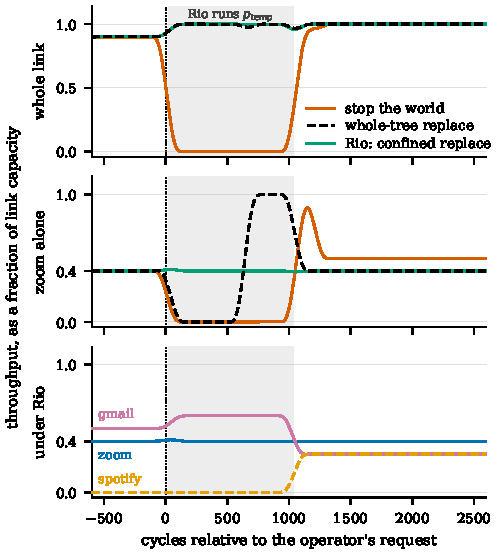
\includegraphics{fig-eval-motivating.pdf}
\caption{The transition of \cref{sec:tour}, as a share of link capacity. The lower panel is just \textsf{zoom}, which the transition request ought not affect. The gray band is the interval in which Rio runs $p_\text{temp}$.}
\label{fig:eval-motivating}
\end{figure}

\paragraph{The baseline}

A switch that stops to reconfigure can do many things with the traffic that arrives meanwhile, and how bad each one is depends on the deployment.
Rather than measure chaos, we remove it from the comparison.
Our stop-the-world baseline is constructed to be lossless and order-preserving: it freezes admission and dequeue, captures the metadata of every buffered packet, installs the target configuration, and replays exactly one scheduler token per captured packet.
Its sources keep generating while it is stopped, and we give it an unbounded input queue, so it never drops a packet when stopped.

We also give the baseline a short period of stoppage: 1024 cycles, a little over a microsecond at the rate of one nanosecond per cycle.
Reconfiguring the program that a running switch executes has been reported at around half a second~\cite{Xing22}, so this is far shorter than any published figure.

\paragraph{The transition of \cref{sec:tour}}

Our first experiment considers exactly the transition that \cref{sec:tour} walks through.
Three mechanisms take the scheduler from \(p_1\) to \(p_2\) over one 2136-packet trace.
The first is the stop-the-world baseline.
The other two are both Rio's.
\emph{Root-level replace} is the fallback described in \cref{sec:sequences}: it builds \(p_2\) beside the running tree, puts the running tree on the high-priority arm of a \(\Strictstar\), and drains it there.
\emph{Confined replace} is the path the planner prefers, which does the same thing at the deepest slot that changed, so only \textsf{gmail}'s subtree sits behind the wrapper.
Throughout, \textsf{zoom} sends enough packets to fill 40\% of the link.
\textsf{gmail} sends enough to fill 80\% before the request and 20\% after it, and \textsf{spotify} starts sending when the request arrives, enough to fill 20\%.
Before the request the three together ask for more than the link can carry, so there is a backlog of packets when the request arrives.

\begin{table}[t]
\centering
\small
\begin{tabular}{lrrr}
\toprule
& Install & Install & Peak \textsf{zoom} \\
Mechanism & Instrs & Cycles & Delay (Cycles) \\
\midrule
stop the world & 25 & 43 & 1050 \\
root-level replace & 26 & 35 & 411 \\
\textbf{confined replace (Rio)} & \textbf{16} & \textbf{28} & \textbf{23} \\
\bottomrule
\end{tabular}
\caption{Install cost and \textsf{zoom}'s peak delay under the three mechanisms that carry \(p_1 \to p_2\) as described in \cref{sec:tour}.}
\label{tab:eval-motivating}
\end{table}

\Cref{fig:eval-motivating} separates two ways a transition can go wrong.
Stopping the scheduler empties the link, so it drops to zero for as long as the stop lasts.
Root-level replace looks better since it keeps the link busy, but the lower panel reveals what it is busy with: it starves \textsf{zoom} for some 300 cycles and then hands it the whole link to catch up.
We know that \textsf{zoom} sits at the same priority and sends the same rate of traffic in every policy here, and yet only Rio gives consistent service to \textsf{zoom}: our peak delay for \textsf{zoom} is 23 cycles, one more than the 22 it sees under a transition that never touches its subtree at all.
Root-level replace costs it 411 and the baseline 1050 (\cref{tab:eval-motivating}), and neither of them recovers when its interval ends: the baseline is still running above its offered rate 3500 cycles after a stop that lasted 1024 cycles.

\begin{figure}[t]
\centering
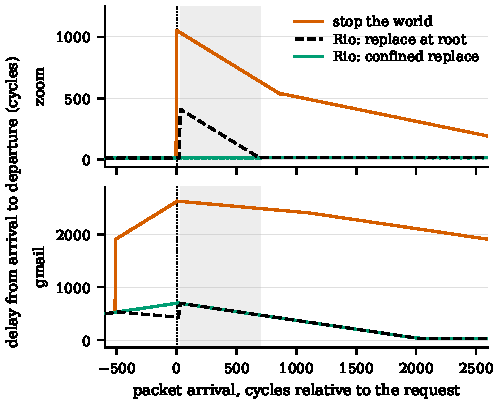
\includegraphics{fig-eval-delay.pdf}
\caption{Delay from arrival to departure, per packet. The upper panel is \textsf{zoom} and the lower is \textsf{gmail}, which holds the backlog.}
\label{fig:eval-delay}
\end{figure}

\cref{fig:eval-delay} shows how long a packet waits between arrival and departure; the request arrives at cycle 0.
The last \textsf{gmail} packet enqueued before the request waits 2618 cycles under the baseline, 433 under root-level replace and 694 under confined replace.
Root-level replace again looks good, but the \textsf{zoom} panel reveals the problem: it clears the backlog quickly because it hands the whole link to the old tree, at \textsf{zoom}'s expense.
Under confinement, \textsf{gmail}\textsubscript{old} takes its own 670-cycle drain and no more.

The gray band in both figures is the interval in which the switch runs \(p_\text{temp}\), the transitional policy the planner discovered on the way to \(p_2\), and its two edges are the two atomic steps of \cref{sec:tour}.
Rio's first step takes effect 28 cycles after the request, at the left edge, where the \(\Strictstar\) node appears above \textsf{gmail}\textsubscript{old} and the freshly built \RR{} subtree.
That step is the cheapest install of the three, since it rewrites one subtree and leaves the rest of the control addressed as it was.
\textsf{gmail}\textsubscript{old} runs empty 696 cycles after the request, the drain guard of \cref{sec:sequences} becomes true, and the second step collapses the \(\Strictstar\) six cycles later at the right edge.
The band is 674 cycles wide, which is two thirds of the baseline's stop. Further, it costs the traffic nothing: the link stays full and \textsf{zoom} is undisturbed from one end of it to the other.
\xxx[am]{Want to point to \Cref{app:ptemp} from here?}

\paragraph{The value of a survivor link}

\(\Strictstar\) exists so that a transitional policy can prefer buffered packets to new ones without moving them.
Any other way of expressing that preference has to put the backlog inside a newly built node, which means writing one scheduler token per buffered packet while the scheduler is stopped.
Our second experiment measures the same transition three ways, across backlogs from 0 to 341 packets standing at the request.
There are two ways to build such a node, and we measure both.
One reserves a spare processing element and fills it with a token for each buffered packet, which stops the scheduler for 0.991 cycles per packet.
The other copies the old subtree onto fresh processing elements, which stops it for 2.969 cycles per packet.
Rio's survivor link stops it for \emph{no time}, no matter how big the backlog, because it is a pointer rather than a place to put packets.
The slope matters more than the constant: without \(\Strictstar\), the price of a transition is determined by how busy the switch was when the request arrived.
This is also why \textsf{spotify} waits for the drain in \cref{app:ptemp}, since Rio declines to relocate the packets already queued and lets them drain in place instead.

\paragraph{Scaling in the size of the tree}

\begin{figure}[t]
\centering
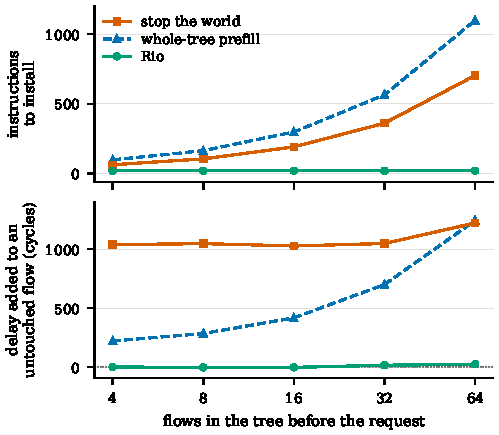
\includegraphics{fig-eval-scaling.pdf}
\caption{Admitting one new tenant, as the tree it joins grows. The lower panel is measured against the same tree already running the target policy.}
\label{fig:eval-scaling}
\end{figure}

Our third experiment holds the request fixed and grows the tree.
The tree runs \WFQ{} over \(m\) tenants, each tenant a two-flow subtree with its own discipline, and we dial up \(m\) from 2 to 32 so the tree holds 4 to 64 flows.
Offered load stays at 1.10 of the link at every point and is spread evenly over the flows, so the congestion does not change with the tree.
The transition request in each case is to \(\Add\) a single tenant at the root.

Rio accomplishes this via the same 21 instructions at every point of the sweep (\cref{fig:eval-scaling}), and finishes in 44 cycles on the smallest tree and 45 on the largest.
Whole-tree prefill goes from 99 instructions to 1099 and stop-the-world reset from 64 to 704, because both reinstall every tenant whether the request named it or not.
Rio never stops the scheduler at any point of the sweep.
% We ran the sweep a second time with a single \(\ChangeMeta\) in place of the \(\Add\), and Rio is flatter still, at 2 instructions and 14 cycles on every tree.

The lower panel measures a flow that the request does not touch, against the same tree already running the target policy.
Rio costs that flow nothing on the three smallest trees, 15 cycles on the next and 24 on the largest tree.
Prefill costs it 221 cycles on the smallest tree and 1242 on the largest.
Stop-the-world sits near 1030 cycles until the largest tree: the 1024-cycle stop we grant it dominates everything else, and only at 64 flows does the cost of rebuilding overtake it.

\paragraph{A larger reconfiguration}

Our fourth experiment considers a request that changes several things at once.
We set up a fourteen-flow tree on seven processing elements, and we change its policy to reweight two tenants, admit four more, and retire one.
No single edit does all of that, so the transition planner decomposes the request into a sequence, and part of that sequence has to wait: the tenant being retired still holds packets, and the guard on its \(\Remove\) does not become true until they have drained (\cref{sec:sequences}).
Rio installs the five unguarded edits in 51 instructions and the guarded \(\Remove\) in 20 more, against 152 for the reset baseline and 201 for whole-tree prefill.
Rio does not stop the scheduler at all, and the two baselines buffer 571 and 424 packets during theirs, which they can do only because we gave them unbounded input queues.
\xxx[am]{Zhiyuan requested a timeline-style figure here but idk if we have the room, and idk if it's punchy enough. Happy to discuss more.}

\paragraph{Hardware cost}

\begin{table}[t]
\centering
\small
\begin{tabular}{rrrr}
\toprule
& \multicolumn{3}{c}{Overhead of Rio's Additions} \\
\cmidrule(l){2-4}
vFlows & LUTs & Registers & BRAM \\
\midrule
32 & 0.1\% & 0.1\% & 32\% \\
128 & 0.9\% & 1.5\% & 36\% \\
512 & 1.5\% & 0.1\% & 41\% \\
1024 & 3.2\% & 0.2\% & 43\% \\
\bottomrule
\end{tabular}
\caption{Synthesis overhead on a Xilinx XCKU5P, five processing elements, 1024 PIFO entries each. Each figure is a percentage of the same design without Rio's additions.}
\label{tab:eval-resources}
\end{table}
\xxx[zhiyuan]{for the table we can also note percentage of hardare resources on FPGA}

We synthesized the scheduler with and without Rio's additions for a Xilinx XCKU5P, sweeping the number of virtual flows the tables must address (\cref{tab:eval-resources}).
The additions cost little logic: at most 3.2\% more LUTs and 1.5\% more registers across a thirty-two-fold range in flow count.
They are paid for in memory, at 32\% to 43\% more block RAM, and the reason is the second table bank of \cref{sec:hw-commit}: making an update atomic means holding a second copy of what the update rewrites.
These figures are sums of synthesized components without placement or routing, so they are not a timing closure, and the denser rows of \cref{tab:eval-resources} exceed the part's own memory.

\section{Related Work}\label{sec:related}

\paragraph{Consistent network update}

One category of related work concerns reconfiguring
packet \emph{forwarding} pipelines (as opposed to scheduling, in this paper).
Several approaches address applying consistent updates across an entire network.
\citet{Reitblatt12} use a versioning scheme:
they label packets according to the version of the network they should see.
\citet{Namjoshi24} instead sequence changes so that route consistency holds with a single table edited in place.
\citet{Mahajan13} study the dependencies that a consistency property imposes among rule updates, and find that stronger properties induce more intricate dependencies and therefore slower updates.
Rio seeks per-packet consistency for each of its edits, inside a single packet scheduler rather than across a network.
Versioning does not carry over to a scheduler, which holds packets whose ranks were fixed when they were \push{}ed.

FlexCore~\cite{Xing22} aims to consistently reconfigure the P4 program running on a programmable switch.
It computes a reconfiguration script, which is a sequence of atomic graph edits that transforms the old program into the new one.
It offers three consistency guarantees that may govern the intermediate states visible between the two endpoints.
Rio similarly works by generating a series of atomic edits to transform one packet-scheduling policy into another (\cref{sec:sequences}).
Every intermediate state during a Rio update is a legible program in the same language that the user writes to specify policies (\cref{thm:interplay}).
FlexCore's strongest guarantee, \emph{program consistency}, lets no intermediate state reach a packet, and a Rio transaction provides that for a single \(\delta\) (\cref{sec:hw-commit}).
Relatedly, \citet{Yang24} demonstrate a system for installing P4 programs on programmable switches without disrupting traffic.

Rio's focus on packet schedulers, as opposed to forwarding pipelines, leads to different techniques.
The primary difference is state.
Packet schedulers are fundamentally stateful:
PIFOs hold in-flight packets,
and each scheduling policy has its own bookkeeping.
State is less fundamental in packet forwarding; for example, FlexCore does not support stateful programs.
Rio therefore has the additional challenge of preserving the state reflecting past packets while reconfiguring the policy for future packets.

\paragraph{Reconfiguring a live scheduler}

Loom~\cite{Stephens19} is a NIC packet scheduler that supports dynamic reconfiguration.
Configuration values travel inline with packet descriptors, and each pipeline stage saves the values to its local memory.
A descriptor and the configuration it carries therefore reach each stage together, which is the effect Rio obtains by delay-aligning commit signals across PEs (\cref{sec:hw-commit}).
Loom does not address the effects on in-flight packets or attempt to offer consistent views during reconfiguration.

SP-PIFO~\cite{Alcoz20} can change the mapping from packet ranks to a fixed set of strict-priority queues as traffic shifts.
Its goal is to minimize the error with respect to an ideal PIFO, i.e., the policy that the operator wrote.
Rio instead focuses on changing the policy itself.

\citet{Alcoz23} raise the question of scheduler reconfiguration.
Their scheduling hypervisor deploys per-tenant scheduling policies onto one switch, and they ask how to move from one such policy to another as tenants arrive and depart.
They name two obstacles: emptying the buffers and resetting the state of the scheduling functions, and leave the mechanism to future runtime-programmable data planes.
Rio answers the first by draining rather than dropping packets (\cref{sec:quiesce}) and the second by declining to reset (\cref{sec:changemeta}).

Reconfiguration is routine in the schedulers deployed at hosts and NICs.
Loom updates rate limiters whenever a VM or a flow starts or stops~\cite{Stephens19}.
PicNIC reacts to a breakdown of isolation between tenants at sub-millisecond timescales~\cite{Kumar19}.
FairNIC gives each tenant an independent subtree of packet schedulers to configure~\cite{Grant20}, so the set of tenants fixes the shape of the tree.
Carousel shapes tens of thousands of flows and policies on a single server~\cite{Saeed17}.
Eiffel argues for scheduling in software on the grounds of a shorter development cycle~\cite{Saeed19}.

\paragraph{Programmable packet scheduling}
% \xxx[as]{I am avoiding ``substrate'' in favor of ``packet scheduler'' because this will be more recognizable to experts. ``Substrate'' is kinda solipsistic; a packet scheduler is only a substrate from Rio's perspective.}

\xxx[as]{Can we replace this entire paragraph with: PIFO trees for packet scheduling were introduced in \citet{Sivaraman16}. Subsequent work has explored tweaks to the PIFO tree model and offered efficient hardware implementations~\cite{Shrivastav19,Alcoz20,Alcoz25,Mostafaei25,Yao23,Atre24,Gao22,vPIFO}.}
\xxx[am]{Yes, but it's quite terse, and it makes it so that we situate the reader a little less. I'll save that cut in case we really need it.}
\citet{Sivaraman16} introduce the PIFO and the PIFO tree for efficient programmable packet scheduling.
PIEO generalizes the primitive to extraction from an arbitrary position in the queue~\cite{Shrivastav19}.
SP-PIFO approximates a PIFO with a stack of strict-priority queues on devices that ship today~\cite{Alcoz20}.
PACKS approximates a PIFO's scheduling order together with its admission control, where earlier approximations captured one at a time~\cite{Alcoz25}.
Exp-PIFO approximates one with adaptive exponential bins, keeping two memory cells of state~\cite{Mostafaei25}.
BMW Tree implements one as a balanced multi-way sorting tree that scales to large flow counts~\cite{Yao23}.
BBQ reaches hundreds of thousands of concurrent flows by carrying hierarchical find-first-set into a pipelined integer priority queue~\cite{Atre24}.
Gearbox approximates weighted fair queuing with a hierarchy of queuing levels at constant cost per operation~\cite{Gao22}.
vPIFO virtualizes a single physical PIFO into many instances that it can wire into a tree of any shape~\cite{vPIFO}.
Its Scheduling Description Language compiler generates that wiring offline, so the shape is fixed before traffic arrives, and vPIFO names runtime updating as future work.
Our policy language is a formal core of theirs (\cref{sec:policy-dsl}).

All of these designs fix the tree's shape and the discipline at each node when the scheduler is configured.
Instead of focusing on the PIFO tree implementation itself, Rio aims to extend any PIFO tree design with run-time reconfiguration.

One recent design offers more than Rio assumes.
UIFO adds a level of classes above packets, so that the service order of already-buffered traffic can be updated after the fact~\cite{Wang26}.
Rio's edits are defined against a substrate where a rank is fixed at \push{} time (\cref{sec:controls}), and our non-disruption theorem (\cref{thm:nondisruption}) is stated against that.
A scheduler that can re-rank a backlog may admit ``retroactive'' reconfigurations that Rio does not consider.

\citet{Mohan23} give a syntax and an operational semantics for PIFO trees.
Our runtime model (\cref{sec:controls}) is adapted from theirs.
\citet{Mittal16} ask whether a single scheduling algorithm can replay the schedule that any other algorithm produced, and find that in general none can.
That work compares two schedulers using the sequence of packets they emit, which is how we compare scheduling policies across an edit (\cref{thm:nondisruption}).

\section{Conclusion}\label{sec:concl}

Reconfiguring a packet scheduler inevitably entails some period of chaos:
when the effective scheduling behavior follows neither the old policy nor the new policy.
Rio rigorously defines the semantics of that transitional period.

\bibliographystyle{ACM-Reference-Format}
\bibliography{main}

\appendix

\section{Edit Semantics}\label{sec:edit-semantics-full}

This appendix lists the full denotational semantics of policy edits, $\delta$.
We define both $\psem{\delta}$ for the effect on high-level policy trees
and $\csem{\delta}$ for the effect on PIFO tree state.

\paragraph{Notation}

Besides \(\mathit{ts}[t/i]\) of \cref{sec:edit-semantics}, we write \(\mathit{ts}[i]\) for the \(i\)-th annotated arm of a \pol node's child list, and \(\mathit{ts}[-/k]\) for \(\mathit{ts}\) with its \(k\)-th arm dropped and later arms shifted one slot to the left.
Control nodes are written \(\langle\mathit{state}, \mathit{pifo}, \mathit{z}\rangle(\mathit{cs})\), and we reuse \(\mathit{cs}[C'/i]\) and \(\mathit{cs}\mathbin{+\!\!+}[C']\) on the child list \(\mathit{cs}\).
Indices follow the \pth convention of \cref{sec:delta-grammar}.

One invariant links a node's classifier to the tree, and every form below preserves it.
At any node, \(\mathrm{dom}(\mathit{z}.\mathit{serves})\) is the set of flows served by the leaves beneath it, and \(\mathit{z}.\mathit{serves}\) sends each of them to the child that leads towards its leaf.

Several forms address the target's parent rather than the target, and split the given path as \(\pi \mathbin{+\!\!+} [k]\): \(\pi\) is the path to the parent, and \(k\) is the child index by which the parent reaches the target.
Paths are also ordered by prefix, with \(\nu \sqsubset \tau\) saying that \(C@\nu\) is a proper ancestor of \(C@\tau\), and \(\nu \sqsubseteq \tau\) allowing \(\nu = \tau\) as well.

Most forms edit only the node that their path points to.
For such a form we use a small combinator: given a node transformer \(g\) and a path \(\pi\), write \(\mathtt{at}(\pi, g)\) for the operation that walks to the node at \(\pi\), applies \(g\) there, and copies every other node of the tree unchanged:
\[
\begin{array}{@{}l@{}}
\mathtt{at}([\,], g)\,(N) = g(N)\\
\mathtt{at}(i \mathbin{::} \mathit{rest}, g)\,\langle\mathit{state},\mathit{pifo},\mathit{z}\rangle(\mathit{cs}) =\\
\quad \langle\mathit{state},\mathit{pifo},\mathit{z}\rangle(\mathit{cs}[\,\mathtt{at}(\mathit{rest}, g)(\mathit{cs}[i]) / i\,])
\end{array}
\]
The same combinator serves on \pol, where a node is \(D(\mathit{ts})\) and the descent into arm \(i\) rewrites that arm's policy and carries its annotation along.
We also write \(\mathtt{at}(V, g)\) for the set analogue, applying \(g\) at every node in \(V\) and copying every node outside \(V\) unchanged.

\Cref{sec:edit-semantics}'s \(\mathtt{extend}\) and \(\mathtt{setmeta}\) recur across the forms, and are given in full here.
A node's discipline fixes a packet's rank from the local \stt and the chosen child alone, not from the packet itself, so admitting a flow at an already-running node calls for no new rank rule, and \(\mathtt{extend}\) therefore touches the classifier and nothing else:
\[
\begin{array}{@{}l@{}}
\mathtt{extend}(\mathit{z}, F, i).\mathit{serves} = \mathit{z}.\mathit{serves}\,[\,f \mapsto i \;\text{for}\; f \in F\,],\\[3pt]
\mathtt{extend}(\mathit{z}, F, i).\mathit{admit} = \mathit{z}.\mathit{admit} \cup F,\\[3pt]
\mathtt{setmeta}(\mathit{z}, i, m).\mathit{meta} = \mathit{z}.\mathit{meta}\,[\,i \mapsto m\,].
\end{array}
\]
Other fields of \zz are carried through unchanged.
A form that admits a new set of flows must extend every node on the way down to its target, so \(\mathtt{extend}\) is also applied as a walk.
At each proper ancestor \(C@\nu\) of the target \(C@\tau\) the walk replaces \zz by \(\mathtt{extend}(\mathit{z}, F, i)\), where \(i\) is the index by which \(\nu\) continues toward \(\tau\), and it copies every other node unchanged.

\Add{} comes first and is given in full detail.
The five that follow lean on it, and we point out only where each one departs from \Add's pattern.

\subsection{\texorpdfstring{\(\Add(\pi, D, \mathit{arm}, m)\)}{Add}}\label{sec:add}


\Add{}'s arguments are \(\pi : \mathit{path}\), the node that will receive the new arm as its last child; \(D\), the discipline that node runs; \(\mathit{arm} : \mathit{pol}\), the policy of the new arm; and \(m \in M_{D}\), the metadatum that tells \disc how to schedule that arm (\cref{sec:policy-dsl}).

\paragraph{Definition}

\(\csem{\Add(\pi, D, \mathit{arm}, m)}(C)\) is defined when four things hold: the path \(\pi\) resolves in \(C\) to an internal node, that node runs the discipline \disc the form names, the metadatum \(m\) is drawn from \(M_{D}\), and \arm's leaf labels are disjoint from those of \(C\).

We define \(\csem{\Add}\) by recursion on \(\pi\), writing \(\mathtt{flows}(\mathit{arm})\) for the set of flows at \(\lceil \mathit{arm} \rceil\)'s leaves:
{\small
\[
\begin{array}{@{}l@{}}
\csem{\Add([\,],\ D,\ \mathit{arm},\ m)}\ \langle\mathit{state},\mathit{pifo},\mathit{z}\rangle(\mathit{cs}) \;=\\
\quad \langle\mathit{state'},\mathit{pifo},z'\rangle(\mathit{cs}\mathbin{+\!\!+}[\lceil\mathit{arm}\rceil])\\
\quad \textbf{where}\ k=|\mathit{cs}|\\
\quad \phantom{\textbf{where}}\ \mathit{state'}=(\mathit{node\_state},\ \mathit{slot\_states}\mathbin{+\!\!+}[s])\\
\quad \phantom{\textbf{where}}\ s=\mathit{init\_slot\_state}_{D}(\mathit{node\_state},m)\\
\quad \phantom{\textbf{where}}\ z'=\mathtt{setmeta}(\mathtt{extend}(\mathit{z},\mathtt{flows}(\mathit{arm}),k),k,m)\\[8pt]
\csem{\Add(i\mathbin{::}\mathit{rest},\ D,\ \mathit{arm},\ m)}\ \langle\mathit{state},\mathit{pifo},\mathit{z}\rangle(\mathit{cs}) \;=\\
\quad \langle\mathit{state},\mathit{pifo},z'\rangle(\mathit{cs}[\,c/i\,])\\
\quad \textbf{where}\ c=\csem{\Add(\mathit{rest},\ D,\ \mathit{arm},\ m)}(\mathit{cs}[i])\\
\quad \phantom{\textbf{where}}\ z'=\mathtt{extend}(\mathit{z},\mathtt{flows}(\mathit{arm}),i)
\end{array}
\]
}
The arguments \disc, \arm, and \(m\) thread unchanged through the recursion, and \(m\) is consumed only at the base case, which annotates the new slot and seeds its bookkeeping.
Because \(\mathtt{flows}(\mathit{arm})\) lies outside \(\mathrm{dom}(\mathit{z}.\mathit{serves})\), every \(\mathtt{extend}\) along the way is conflict-free.
The recursive case is exactly the \(\mathtt{extend}\) walk of \cref{sec:edit-semantics}, carrying \(\mathtt{flows}(\mathit{arm})\) down to \(\pi\).
Appending the arm at the base case is legitimate because our arm-order freedom (\cref{sec:policy-dsl}) lets us place the new child last.

\paragraph{Pol-level reading}

We define \(\psem{\cdot}\) by recursion on \(\pi\) as well:
{\small
\[
\begin{array}{@{}l@{}}
\psem{\Add([\,],\ D,\ \mathit{arm},\ m)}\ (D\ \mathit{ts}) \;=\; D(\mathit{ts}\mathbin{+\!\!+}[m{:}\,\mathit{arm}])\\[4pt]
\psem{\Add(i\mathbin{::}\mathit{rest},\ D,\ \mathit{arm},\ m)}\ (E\ \mathit{ts}) \;=\\
\quad E(\mathit{ts}[\,\psem{\Add(\mathit{rest},\ D,\ \mathit{arm},\ m)}(\mathit{ts}[i])/i\,])
\end{array}
\]
}
The metadatum \(m\) appears on both sides.
\(\csem{\Add}\) records it at \(\mathit{z}.\mathit{meta}(k)\), and \(\psem{\Add}\) writes it onto the new arm, so reading the edited control back recovers the annotation the operator asked for.

\subsection{\texorpdfstring{\(\ChangeMeta(\tau, D, m)\)}{ChangeMeta}}\label{sec:changemeta}


\ChangeMeta{} re-tunes a single already-running arm, resetting the metadatum its parent schedules it by, without moving a packet or disturbing any sibling.
Its path is non-empty and destructs as \(\pi \mathbin{+\!\!+} [k]\), so \(k\) is the arm's slot at its parent \(C@\pi\); \disc is the discipline the parent runs, and \(m\) is a fresh value from \(M_{D}\).
Carrying \disc on the form makes \(m \in M_{D}\) checkable from the form alone, rather than only against the control it is about to be applied to.

\ChangeMeta{} is defined when \(\tau\) resolves in \(C\) to an arm whose parent runs the \disc the form names, when \(m \in M_{D}\), and when that parent's ranker does not name \(\Strictstar\).
Changing the metadata of a \(\Strictstar\) is illegal, and \cref{sec:hw-survivor} turns that to account: a node whose priorities cannot change needs no \pifo of its own.
Its node transformer \(\mathtt{setmeta}_k\) rewrites the node's \zz and nothing else:
{\small
\[
\mathtt{setmeta}_k\ \langle\mathit{state},\mathit{pifo},\mathit{z}\rangle(\mathit{cs}) = \langle\mathit{state},\mathit{pifo},\ \mathtt{setmeta}(\mathit{z},k,m)\rangle(\mathit{cs}).
\]
}
The form applies that transformer at the parent and nowhere else:
\[
\csem{\ChangeMeta(\pi \mathbin{+\!\!+} [k],\, D,\, m)} = \mathtt{at}(\pi,\, \mathtt{setmeta}_k).
\]
Under \Strict{} the arm's metadatum is its priority, and under \WFQ{} it is its weight; that value alone becomes \(m\), and the evolving per-arm bookkeeping beside it is left untouched.
At \pol-level, \ChangeMeta{} reannotates arm \(k\) and leaves that arm's policy, its siblings, and the discipline \disc alone:
\[
\begin{array}{@{}l@{}}
\psem{\ChangeMeta(\pi \mathbin{+\!\!+} [k],\, D,\, m)} =\\[3pt]
\quad \mathtt{at}\big(\pi,\; D(\ldots, m_k{:}\,t_k, \ldots) \mapsto D(\ldots, m{:}\,t_k, \ldots)\big).
\end{array}
\]

That is the line \cref{sec:controls} draws between the configuration the operator chose and what serving traffic left behind.
Resetting the bookkeeping would pull the targeted arm out of the round in progress, rewarding or penalizing it for no reason the operator asked for.
Whatever \disc keeps beside the metadatum belongs to \disc (\cref{sec:compilation}), and a re-tuning does not touch it.
A discipline that keeps no per-arm bookkeeping, such as \Strict, does not raise the question.

\subsection{\texorpdfstring{\(\Quiesce(\tau)\)}{Quiesce}}\label{sec:quiesce}


\Quiesce{} strikes every flow served under \(C@\tau\) from the admitted sets of the nodes those flows traverse, so that no packet bound for a leaf there is admitted anywhere, while leaving every node's routing in place so buffered packets can still be popped out.
This is the payoff of keeping \(\mathit{z}.\mathit{admit}\) separate from \(\mathrm{dom}(\mathit{z}.\mathit{serves})\) (\cref{sec:controls}): a silenced flow leaves the admitted set while its entry in the service map stays.
This is the only way the containment \(\mathit{z}.\mathit{admit} \subseteq \mathrm{dom}(\mathit{z}.\mathit{serves})\) becomes strict, and only \Remove{} deletes the mapping itself.

\(\csem{\Quiesce(\tau)}(C)\) is defined whenever \(\tau\) resolves in \(C\) (the empty path silences the whole tree).
Let \(L = \mathtt{flows}(C@\tau)\) be the flows to silence.
Write \(\mathit{z} \setminus L\) for \zz with \(L\) struck from its admitted set, so \((\mathit{z} \setminus L).\mathit{admit} = \mathit{z}.\mathit{admit} \setminus L\).
Its service map and its ranker are unchanged.
The nodes that those flows traverse are the spine down to \(\tau\) together with \(\tau\)'s whole subtree:
\[
V_\tau = \{\, C@\nu \;:\; \nu \sqsubseteq \tau \,\} \;\cup\; \{\, \text{every node of } C@\tau \,\}.
\] 
\Quiesce{} narrows the admitted set at each of these nodes and touches nothing else, through the node transformer
\[
g_L\ \langle\mathit{state},\mathit{pifo},\mathit{z}\rangle(\mathit{cs}) = \langle\mathit{state},\mathit{pifo},\ \mathit{z} \setminus L\rangle(\mathit{cs}),
\]
applied at every node of \(V_\tau\):
\[
\csem{\Quiesce(\tau)} = \mathtt{at}(V_\tau,\ g_L).
\]
The restriction has to reach every node of \(V_\tau\) rather than the root alone.
Under \cref{sec:controls}'s parallel \push{}, every node on the path from the system root to a packet's destination leaf mints an index via its local \zz independently of the others.
If we restricted \zz at only a subset of those nodes, say only the root or only inside \(C@\tau\), the rest would go on minting indices and enqueueing them, the tree would be malformed, and a later \pop{} would get stuck.

At \pol-level, \(\psem{\Quiesce(\tau)}\) is the identity.

\subsection{\texorpdfstring{\(\Remove(\tau)\)}{Remove}}\label{sec:remove}

As before, \(\tau : \mathit{path}\) is the non-empty target arm; destruct it as \(\pi \mathbin{+\!\!+} [k]\).
\Remove{} unhooks that arm and renumbers higher siblings down by one; it fires only when the arm's subtree is empty (see note below).

\paragraph{Definition}

As in \cref{sec:quiesce}, let \(L = \mathtt{flows}(C@\tau)\), here the flows that the doomed arm serves.
Write \(\mathit{z} \dsetminus L\) for \zz with \(L\) struck from its service map, and hence, by the containment of \cref{sec:controls}, from its admitted set too.
Its ranker is unchanged.
\Remove{} drops the arm at its parent and strikes \(L\) from the service map of every proper ancestor above that parent, the set \(A_\pi = \{\, C@\nu \;:\; \nu \sqsubset \pi \,\}\).
It is defined when \(\tau\) resolves in \(C\), when the subtree at \(\tau\) is empty, and when \(C@\tau\)'s ranker does not name \(\Strictstar\).
A \(\Strictstar\) node can only be retired by \Undesignate{} (\cref{sec:undesignate}), which promotes the arm beneath it and is the only way \cref{sec:hw-survivor} leaves the substrate to dismantle one.
Dropping arm \(k\) shifts every later arm one slot to the left, and we name that shift \(\sigma_k\): the map on child indices that fixes every \(i < k\) and sends every \(i > k\) to \(i-1\).
The node transformer \(\mathtt{drop}_k\) unhooks child \(k\) and renumbers what named it:
{\small
\[
\begin{array}{@{}l@{}}
\mathtt{drop}_k\ \langle(\mathit{node\_state}, \mathit{ss}),\ \mathit{pifo},\ \mathit{z}\rangle(\mathit{cs}) \;=\\
\quad \langle(\mathit{node\_state},\ \mathit{ss}[-/k]),\ \sigma_k(\mathit{pifo}),\ z'\rangle(\mathit{cs}[-/k])\\
\quad \textbf{where}\ z'.\mathit{serves} = \sigma_k \circ (\mathit{z} \dsetminus L).\mathit{serves}\\
\quad \phantom{\textbf{where}}\ z'.\mathit{admit} = (\mathit{z} \dsetminus L).\mathit{admit}\\
\quad \phantom{\textbf{where}}\ z'.\mathit{meta} = \mathit{z}.\mathit{meta} \circ \sigma_k^{-1}\\
\quad \phantom{\textbf{where}}\ z'.\mathit{rank} = \mathit{z}.\mathit{rank}
\end{array}
\]
}
The form drops the arm at its parent and retracts \(L\) at every proper ancestor:
\[
\csem{\Remove(\pi \mathbin{+\!\!+} [k])} = \mathtt{at}(A_\pi,\ \mathit{z} \dsetminus L) \circ \mathtt{at}(\pi,\, \mathtt{drop}_k).
\]
Emptiness and \(\vdash C\) force \(C@\pi.\mathit{pifo}\) to hold \emph{no entry} equal to \(k\), so \pifo loses no entry, and surviving entries keep their child.

\paragraph{Note: Why the ancestors are retracted too}

Dropping the arm at its parent alone would leave every node above still mapping \(L\) toward it.
A later \push{} of an \(L\)-packet would then be admitted at an ancestor and enqueue an index there, while the parent, which no longer serves \(L\), would enqueue nothing.
This would leave \(\vdash\) broken.

\paragraph{Pol-level reading}

\Remove{} drops arm \(k\) from the parent \pol node:
\[
\psem{\Remove(\pi \mathbin{+\!\!+} [k])} = \mathtt{at}(\pi,\; D(\mathit{ts}) \mapsto D(\mathit{ts}[-/k])).
\]

\paragraph{Note: Why insist on an empty subtree}

\newcommand{\rmpanel}[3]{% #1 P-strikes, #2 Q-strikes, #3 B-struck (0/1)
\begin{tikzpicture}[x=1cm,y=1cm]
  \node (Pp) at (0,0) {\numpifo{0,1,0,1,0,1,0}{#1}};
  \node[font=\scriptsize,anchor=east,inner sep=1.5pt] at (Pp.west) {$P$};
  \node (Qp) at (-0.45,-1.05) {\numpifo{0,0,1,1}{#2}};
  \node[font=\scriptsize,anchor=east,inner sep=1.5pt] at (Qp.west) {$Q$};
  \leaftri{flowB}{0.95}{-0.95}{3}{0}
  \leaftri{flowA}{-0.82}{-1.98}{2}{0}
  \leaftri{flowC}{-0.12}{-1.98}{2}{#3}
  \draw (Pp.south) -- (Qp.north);
  \draw (Pp.south) -- (0.95,-0.95);
  \draw (Qp.south) -- (-0.82,-1.98);
  \draw (Qp.south) -- (-0.12,-1.98);
  % Edge labels: each pair shares a y, and each sits the same perpendicular
  % distance from its own edge, so the shallower right edge takes a larger
  % horizontal offset than the steep left one.
  \node[font=\scriptsize,inner sep=0pt] at (-0.361,-0.53) {0};
  \node[font=\scriptsize,inner sep=0pt] at ( 0.540,-0.53) {1};
  \node[font=\scriptsize,inner sep=0pt] at (-0.734,-1.62) {0};
  \node[font=\scriptsize,inner sep=0pt] at (-0.187,-1.62) {1};
\end{tikzpicture}%
}
\begin{figure}[t]
  \centering
  \captionsetup[subfigure]{justification=raggedright,singlelinecheck=false}
  \begin{subfigure}[t]{0.32\linewidth}\centering\rmpanel{0}{0}{0}\caption{Original.}\label{fig:remove-orig}\end{subfigure}\hfill
  \begin{subfigure}[t]{0.32\linewidth}\centering\rmpanel{5,7}{3,4}{1}\caption{Rightmost 0s struck.}\label{fig:remove-strike-right}\end{subfigure}\hfill
  \begin{subfigure}[t]{0.32\linewidth}\centering\rmpanel{1,3}{3,4}{1}\caption{Leftmost 0s struck.}\label{fig:remove-strike-left}\end{subfigure}
  \caption{Removing \tritext{flowC} forces out \(Q\)'s two index-1 entries and two of \(P\)'s four index-0 entries (struck red). Which two \(0\)s to strike is unspecified, so (b) and (c) are both legal.}
  \label{fig:remove-ambiguity}
\end{figure}
Deleting an \emph{occupied} child has no canonical local realization.
Consider the well-formed tree of \cref{fig:remove-orig}, whose internal nodes are \(P\) and \(Q\), with the annotations on the arms showing how a parent refers to a child.
Say the operator asks us to delete \tritext{flowC}, dropping its packets.
To restore well-formedness, we need to remove two instances of the index \(1\) from \(Q\)'s PIFO and two instances of the index \(0\) from \(P\)'s PIFO.

At \(Q\) the edit is unambiguous.
Well-formedness of the original tree forces \(Q\)'s PIFO to have exactly two instances of \(1\), and we delete those two.
The trouble is one level up.
\(P\)'s PIFO originally had four instances of \(0\), and well-formedness demands that we remove two of them.
But \emph{which} two?
No entry in \(P\) carries the meta-information ``I was enqueued when a packet was inserted into \tritext{flowC}''; an entry \(0\) in \(P\) only means ``when this index is popped, recursively ask subtree \(Q\) to emit the next packet'' (see \cref{sec:background}).
This absence of meta-information is a \emph{feature} of PIFO trees, not a defect: an entry is deliberately detached from the packet it was enqueued with, which lets each node schedule its own discipline in isolation and lets a subtree be reconfigured without rewriting its ancestors.

Given this, there is no obvious or operator-provided answer: whichever two instances of \(0\) we strike, the choice is itself a scheduling decision, since it affects how \(P\) intermixes \tritext{flowB} traffic with \(Q\)'s.
Strike the two rightmost \(0\)s (\cref{fig:remove-strike-right}) and five pops drain \(P\) as \popseq{flowB,flowB,flowA,flowB,flowA}.
Strike the two leftmost instead (\cref{fig:remove-strike-left}) and the same five pops drain it as \popseq{flowA,flowB,flowA,flowB,flowB}.
The \emph{choice of which} \(0\)s to strike \emph{silently reschedules \tritext{flowA} against \tritext{flowB}}, and nothing in the operator's deletion request records what the operator wanted.

We do not wish to make a scheduling decision for the operator, and the only way to avoid one is to drain the whole tree, filter out \tritext{flowC}'s packets, and re-push, which is a stop-the-world rebuild.

Our grammar sidesteps the question entirely, by asking that a targeted subtree be empty before it is deleted (\cref{sec:sequences}).
At the instant \Remove{} fires, no entry above the doomed arm was enqueued on account of a packet inside it, so no entry has to be dropped and the structural deletion is unambiguous.

% Issued before the section head so fig:designate lands on a page A.5
% can reach, rather than after Appendix A has ended.
\begin{figure*}[t]
  \centering
  \begin{subfigure}[t]{0.19\linewidth}
    \centering
    \begin{tikzpicture}[every node/.style={font=\scriptsize}]
      \node (P) at (0,0) {$P$};
      \draw (P) -- (0,-0.75);
      \subtri{oldcol}{0}{-0.75}{3}
    \end{tikzpicture}
    \caption{Before.}
    \label{fig:designate-before}
  \end{subfigure}\hfill
  \begin{subfigure}[t]{0.19\linewidth}
    \centering
    \begin{tikzpicture}[every node/.style={font=\scriptsize}]
      \node (P) at (0,0) {$P$};
      \node (S) at (0,-0.75) {$\Strictstar$};
      \draw (P) -- (S);
      \draw (S) -- (-0.95,-0.75);
      \draw (S) -- (0.95,-0.75);
      \subtri{oldcol}{-0.95}{-0.75}{3}
      \subtri{newcol}{0.95}{-0.75}{0}
    \end{tikzpicture}
    \caption{After \Designate.}
    \label{fig:designate-after}
  \end{subfigure}\hfill
  \begin{subfigure}[t]{0.19\linewidth}
    \centering
    \begin{tikzpicture}[every node/.style={font=\scriptsize}]
      \node (P) at (0,0) {$P$};
      \node (S) at (0,-0.75) {$\Strictstar$};
      \draw (P) -- (S);
      \draw (S) -- (-0.95,-0.75);
      \draw (S) -- (0.95,-0.75);
      \subtri{oldcol}{-0.95}{-0.75}{2}
      \subtri{newcol}{0.95}{-0.75}{3}
    \end{tikzpicture}
    \caption{Mid-drain.}
    \label{fig:designate-drain}
  \end{subfigure}\hfill
  \begin{subfigure}[t]{0.19\linewidth}
    \centering
    \begin{tikzpicture}[every node/.style={font=\scriptsize}]
      \node (P) at (0,0) {$P$};
      \node (S) at (0,-0.75) {$\Strictstar$};
      \draw (P) -- (S);
      \draw (S) -- (-0.95,-0.75);
      \draw (S) -- (0.95,-0.75);
      \subtri{oldcol}{-0.95}{-0.75}{0}
      \subtri{newcol}{0.95}{-0.75}{3}
    \end{tikzpicture}
    \caption{Before \Undesignate.}
    \label{fig:designate-predrop}
  \end{subfigure}\hfill
  \begin{subfigure}[t]{0.19\linewidth}
    \centering
    \begin{tikzpicture}[every node/.style={font=\scriptsize}]
      \node (P) at (0,0) {$P$};
      \draw (P) -- (0,-0.75);
      \subtri{newcol}{0}{-0.75}{3}
    \end{tikzpicture}
    \caption{After \Undesignate.}
    \label{fig:designate-done}
  \end{subfigure}

  \caption{The \Designate\,+\,drain\,+\,\Undesignate{} lifecycle. The doomed subtree is \tritext{oldcol} and the survivor \tritext{newcol}, both under parent \(P\).}
  \label{fig:designate}
\end{figure*}

\subsection{\texorpdfstring{\(\Designate(\tau, \mathit{survivor})\)}{Designate}}\label{sec:designate}


\(\tau : \mathit{path}\) is the path to the target subtree being wrapped, and \(\mathit{survivor} : \mathit{pol}\) is the designated-survivor policy that becomes the new \(\Strictstar\) node's low-priority arm.

Say the presently running control is \(C\).
Intuitively, \Designate{} replaces \(C@\tau\) in place with \(\Strictstar(C@\tau, \lceil \mathit{survivor} \rceil)\).
It is the mechanism behind non-disruptive in-place replacement (\cref{fig:designate}).
The \(\Strictstar\) node lets \survivor begin accepting new traffic on a low-priority arm, while the old subtree keeps draining, on a high-priority one.
Once the old subtree is empty, \Undesignate{} removes it and promotes \survivor in its place.
That is why the form exists: no single edit can swap one subtree for another without either dropping the old subtree's backlog or stalling the new arm, but the \(\Strictstar\) node lets both coexist for the length of a drain.

\Designate{} installs a ranker that names \(\Strictstar\), and \Undesignate{} retires the node carrying it.
A node's ranker records which discipline the node runs (\cref{sec:controls}), so both forms state their preconditions structurally, and no other form disturbs such a node.
That node is visible at \pol-level as a \(\Strictstar\), which is what \(\lfloor \cdot \rfloor\) (\cref{sec:equivalences}) reports of it.
An operator may write a \(\Strictstar\) directly, but one usually arises in the middle of a planner sequence, between a \Designate{} and its eventual \Undesignate.
\cref{sec:hardware} takes up why the two disciplines are kept apart, which turns out to be a question about hardware layout rather than about scheduling.


\paragraph{Definition}

\(\csem{\Designate(\tau, \mathit{survivor})}(C)\) is defined when \(\tau\) resolves in \(C\), and when every flow \survivor serves is one that either nothing in \(C\) serves or that \(C@\tau\) itself serves.
So \survivor may reuse the flows of the subtree it is replacing, and it may introduce new flows, but it may not claim a flow that some other part of \(C\) is already serving.
\cref{fig:designate} draws the target subtree as \tritext{oldcol} and the survivor as \tritext{newcol}.
Write \(M = C@\tau\) for the target, and let \(P_0\) be the number of packets buffered under it (\(P_0 = 3\) in \cref{fig:designate-before}).
\Designate{} wraps the target and admits \survivor's flows at every ancestor on the way down.
That walk is similar to that of \Add, with \survivor's flows in place of the new arm's.
The two differ only at the target, since \Add{} appends an arm there while \Designate{} wraps the node it has reached.
The transformer \(\mathtt{wrap}\) replaces \(M\) with a fresh \(\Strictstar\) node \(N\) over the two arms \([\,M,\ \lceil\mathit{survivor}\rceil\,]\), giving the old arm strict priority over the new arm:
{\small
\[
\begin{array}{@{}l@{}}
\mathtt{wrap}(M) = N = \langle s_N,\ q_N,\ \mathit{z}_N \rangle\big([\,M,\ \lceil\mathit{survivor}\rceil\,]\big),\ \textbf{where}\\[3pt]
\quad n_N = \mathit{init\_node\_state}_{\Strictstar},\\[3pt]
\quad s_N = (\,n_N,\ [\,\mathit{init\_slot\_state}_{\Strictstar}(n_N, \mathtt{hi}),\\
\quad\qquad\qquad\ \ \mathit{init\_slot\_state}_{\Strictstar}(n_N, \mathtt{lo})\,]\,),\\[3pt]
\quad q_N = \text{the \pifo of } P_0 \text{ copies of the entry } (0,\ \mathtt{hi}),\\[3pt]
\quad \mathit{z}_N.\mathit{meta} = \{\, 0 \mapsto \mathtt{hi},\ 1 \mapsto \mathtt{lo} \,\},\\[3pt]
\quad \mathit{z}_N(p) = (1,\ \mathtt{lo})\ \text{if}\ \mathit{flow}(p) \in \mathtt{flows}(\mathit{survivor}),\ \text{else}\ (0,\ \mathtt{hi}).
\end{array}
\]
}
Its ranker names \(\Strictstar\) rather than \Strict, and \cref{sec:undesignate}'s \Undesignate{} later looks for that name.
Arm \(0\) is \(M\) (\textsf{old}), unchanged down to its whole subtree and buffered packets; arm \(1\) is the freshly compiled \(\lceil\mathit{survivor}\rceil\) (\textsf{new}), initially empty (\cref{fig:designate-after}).
\(N\)'s index-\pifo holds one entry per packet buffered under \textsf{old} and none for arm \(1\), so that backlog keeps popping through \(N\) ahead of any later arrival, unchanged, while \textsf{new} fills only as fresh traffic arrives (\cref{fig:designate-drain}).
Because \(\mathtt{at}\) writes \(N\) back into the parent's slot \(k\), the parent's \(\mathit{z}.\mathit{meta}(k)\) is unchanged, so \(N\) is transparent to the parent.
If \(\tau\) is empty the whole control becomes \(N\), with the old root as arm \(0\).

Like \(\csem{\Add}\), the form is a recursion on the path, and only its base case is new:
\[
\csem{\Designate([\,],\ \mathit{survivor})}\ M = \mathtt{wrap}(M).
\]
Its recursive case is \(\csem{\Add}\)'s, carrying \(\mathtt{flows}(\mathit{survivor})\) rather than \(\mathtt{flows}(\mathit{arm})\) down toward \(\tau\).

Overlap of leaf labels between \(C@\tau\) and \survivor is permitted, and the moment when \(\delta\) fires becomes the boundary between old traffic and new.
The two arms thus stay operationally disjoint even when their label sets overlap.

\paragraph{Pol-level reading}

\Designate{} wraps the \pol subtree at \(\tau\):
\[
\begin{array}{@{}l@{}}
\psem{\Designate(\tau, \mathit{survivor})} ={}\\
\quad \mathtt{at}(\tau, t \mapsto \Strictstar(\mathtt{hi}{:}\,t, \mathtt{lo}{:}\,\mathit{survivor})).
\end{array}
\]

\subsection{\texorpdfstring{\(\Undesignate(\tau)\)}{Undesignate}}\label{sec:undesignate}


\Undesignate{} is the structural inverse of \Designate: it drops a \(\Strictstar\) node whose arm 0 is empty, leaving arm 1 behind (the last step of \cref{fig:designate}).
Below we write \(N\) for that node and \(B\) for its surviving arm, both as controls, and \(|B|\) for the number of packets buffered under \(B\).

\Undesignate{} is defined when \(C@\tau\)'s ranker names \(\Strictstar\), and when its arm 0 is empty.
\(\mathtt{unwrap}\) returns arm 1 of the node, \(B\), with its subtree and contents unchanged; the node \(N = C@\tau\) and its empty arm-0 subtree are discarded.
Since \(\mathtt{at}\) writes \(B\) back into the parent's slot \(k\), the parent's \(\mathit{z}.\mathit{meta}(k)\) is unchanged and \(B\) hangs directly where \(N\) did:
\[
\csem{\Undesignate(\tau)} = \mathtt{at}(\tau,\, \mathtt{unwrap}).
\]
At \pol-level the wrapper collapses and its low arm, \(\lfloor B \rfloor\), is left behind:
\[
\psem{\Undesignate(\tau)} = \mathtt{at}(\tau,\; \Strictstar(\mathtt{hi}{:}\,a,\ \mathtt{lo}{:}\,b) \mapsto b).
\]
The wrapper's own annotations go with it, and the surviving arm inherits the annotation the wrapper held at its parent.
The empty-arm-0 precondition is operational and leaves no trace at \pol-level.

\section{Reading a Policy off a Control}\label{app:readback}

We write \(\lfloor C \rfloor\) for the \pol that \(C\) realizes (\cref{sec:equivalences}).
It walks the control's tree and recovers, node by node, the \pol term the control implements, discarding the live \pifo and \stt contents that traffic happens to have left behind.
We define it by structural recursion on \(C\), with one clause for leaves and one for internal nodes.
Both clauses read out of \zz (\cref{sec:controls}).
A leaf is named by the flow its classifier serves.
An internal node is named by the discipline its ranker names, and its arms are annotated out of its metadata.

\[
\begin{array}{@{}l@{}}
\lfloor C \rfloor = f,\ \text{when \(C\) is a leaf and } \mathrm{dom}(\mathit{z}.\mathit{serves}) = \{f\};\\[4pt]
\lfloor C \rfloor = D(m_1{:}\,\lfloor c_1 \rfloor, \ldots, m_n{:}\,\lfloor c_n \rfloor),\\
\qquad \text{when \(C\) is internal with children } c_1 \ldots c_n,\\
\qquad \mathit{z}.\mathit{rank} \text{ names } D, \text{ and } m_i = \mathit{z}.\mathit{meta}(i).
\end{array}
\]

The recursion runs on a finite tree and consults neither \stt nor \pifo nor \(\mathit{z}.\mathit{admit}\), so it returns a single value.
\xxx[AM to AS]{You suggested defining \(\lfloor \cdot \rfloor\) as the inverse of \(\lceil \cdot \rceil\), and then worried that \(\lceil \cdot \rceil\) is not invertible if one is strict about sibling order.
\(\lfloor \cdot \rfloor\) is now a structural recursion on \(C\), so it is total and single-valued by construction, and no inverse has to be argued for.
The two items below are then consequences rather than defining rules, and the agreement of \cref{sec:interplay} is a third.}
\xxx[as]{OK, I see that this is true. But I am not sure what this separate definition (instead of defining it as an inverse) has bought us. It seems to create a new proof obligation, i.e., to prove that the two things happen to be inverses. Let's discuss this.}
Every well-formed control therefore determines one \pol, independently of how that control was reached, and we may write \(\lfloor C \rfloor\) and use it as a function.

Two facts follow.

\begin{enumerate}
\item \emph{Compiler correctness.} Compiling a \(p\) to a control and reading it straight back recovers \(p\) itself, up to the sibling-order freedom the compiler enjoyed in laying it out: \(\lfloor \lceil p \rceil \rfloor \eqR p\).
This is immediate from the compilation of \cref{sec:compilation}, which installs \disc's ranker at each internal node, copies each arm's annotation into \(\mathit{z}.\mathit{meta}\), and has each leaf serve its own flow.
The relation is \(\eqR\) rather than \(=\) precisely because the compiler can choose arm order when creating \(\lceil p \rceil\).
\item \emph{Insensitivity to live contents.} \(\lfloor \cdot \rfloor\) reads only the tree shape, each leaf's served flow, and each internal node's ranker-discipline and per-arm metadata.
It never reads \stt, \pifo, or \(\mathit{z}.\mathit{admit}\).
So \(\sim\)-related controls, which share shape and \zz outright, are equal when read off using \(\lfloor \cdot \rfloor\). 
Thus, if \(C \sim C'\), then \(\lfloor C \rfloor = \lfloor C' \rfloor\).
\end{enumerate}



\section{Proofs}\label{sec:per-form}

This appendix argues the validity of the theorems in \cref{sec:correctness}.
It proves both in one section rather than one section each.
Neither \(\delta\) nor \(\csem{\delta}\) is recursive, so each theorem is a case analysis over the same six forms, and giving each theorem its own section would run that split twice and separate the checks that a single form owes.

Each form owes three checks, and together the six sets of three prove the two theorems above.
The Characterizations have content because each is proved against a \(\lfloor \cdot \rfloor\) fixed in advance, so they are six separate claims rather than six readings of one definition.
Two of the checks feed \cref{thm:interplay}, and the third feeds \cref{thm:nondisruption}.
Throughout, we write \(C\) for the pre-edit control and \(C'\) for the post-edit control, and \(p = \lfloor C \rfloor\), \(p' = \lfloor C' \rfloor\) for the policies they realize.
All three checks assume \(\csem{\delta}(C)\) is defined.
Outside the region \cref{sec:edit-semantics} specifies, \(\csem{\delta}\) is undefined.

\begin{itemize}
\item \emph{Preservation of \(\vdash\).} \(\vdash C\) implies \(\vdash C'\).
Any packets or index entries that \(\csem{\delta}\) drops or adds must leave the per-node pifo and packet counts in balance.
\item \emph{Characterization.} Prove that reading the policy off the edited control agrees, up to \(\eqR\), with applying the \(\psem{\delta}\) of \cref{sec:edit-semantics} to the policy read off the original: \(p' \eqR \psem{\delta}(p)\).
\item \emph{Non-disruption.} A \pop{} reads only \pifo contents: it pops the root index-\pifo to a child, recurses, and finally emits a leaf packet, never consulting any \stt or \zz (\cref{sec:controls}).
So if \(\csem{\delta}\) leaves the contents of every non-empty \pifo of \(C\) unchanged, never rewriting, reordering, or removing a live entry and introducing only empty \pifo{}s, then the backlog survives entry-for-entry and \(\flush(C) = \flush(C')\).
We call the nodes and fields that a form touches its \emph{footprint}, and the check is that the footprint holds no live \pifo entry.
Where a form's footprint does hold one, we argue directly that the \pop{} sequence is unchanged.
\end{itemize}

Fifteen of the eighteen checks are immediate from the rules of \cref{sec:edit-semantics}: they name the fields that a rule writes and observe that the property at issue does not depend on them.
The other three take an argument of their own: \Add's Characterization, and Non-disruption for \Designate{} and \Undesignate.
The six subsections below give all eighteen, in the order \cref{fig:delta-grammar} lists the forms.

\subsection{\texorpdfstring{\Add}{Add}}\label{sec:check-add}

\paragraph{Preservation of \(\vdash\)}
No pre-existing entry can name the new slot \(k\), and \(\lceil \mathit{arm} \rceil\) compiles empty, so slot \(k\) counts \(0 = 0\).
Every other slot inherits its count.

\paragraph{Characterization}
Both recursions descend \(\pi\) in the same shape, so we induct on \(\pi\).
At the base (\(\pi = []\)), \(\psem{\cdot}\) appends the annotated arm \(m{:}\,\mathit{arm}\), while \(\csem{\Add}\) appends \(\lceil \mathit{arm} \rceil\) at slot \(k\) and sets \(\mathit{z}.\mathit{meta}(k)\) to \(m\).
We have \(\lfloor \lceil \mathit{arm} \rceil \rfloor \eqR \mathit{arm}\), and \(\lfloor \cdot \rfloor\) reads the annotation back off \(\mathit{z}.\mathit{meta}\).
So the two agree on the new arm up to \(\eqR\), and every existing arm is untouched.
At a recursive step, both descend into child \(i\) and write the result back, so the claim follows from the induction hypothesis.
The ancestor itself adds nothing to reconcile.
\(\csem{\Add}\) leaves its \stt and \pifo unchanged, and its \zz-extension is confined to the classifier of an internal node, which \(\lfloor \cdot \rfloor\) does not read.
So the two sides agree all the way down the spine and can differ only inside \(\lceil \mathit{arm} \rceil\), where sibling order is free; that is exactly the \(\eqR\)-slack the claim allows, giving \(p' \eqR \psem{\Add(\pi, D, \mathit{arm}, m)}(p)\).

\paragraph{Non-disruption}
The footprint is the empty slot \(k\), its metadatum, the empty \(\lceil \mathit{arm} \rceil\), and the on-path \zz-extensions.
A \zz-edit changes no \pifo, so none of these is a live entry.

\subsection{\texorpdfstring{\ChangeMeta}{ChangeMeta}}\label{sec:check-changemeta}

\paragraph{Preservation of \(\vdash\)}
The footprint is one \(\mathit{z}.\mathit{meta}\) entry, so no child, no \pifo, and no count moves.

\paragraph{Characterization}
No arm changes position, so the two sides agree exactly rather than up to \(\eqR\): \(p' = \psem{\ChangeMeta(\tau, D, m)}(p)\).

\paragraph{Non-disruption}
An entry's rank was fixed when it was \push{}ed, so the new metadatum governs future pushes only.

\subsection{\texorpdfstring{\Quiesce}{Quiesce}}\label{sec:check-quiesce}

\paragraph{Preservation of \(\vdash\)}
Only the admitted sets across \(V_\tau\) narrow.
Every \pifo, child, and \stt is untouched.

\paragraph{Characterization}
\(\lfloor \cdot \rfloor\) does not read \(\mathit{z}.\mathit{admit}\), and \(\mathit{z}.\mathit{serves}\) is left in place, so a silenced leaf keeps its identity and \(\psem{\Quiesce(\tau)}\) is the identity.

\paragraph{Non-disruption}
Packets already buffered under \(C@\tau\) keep their entries and still drain.
Only future \push{}es are refused.

\subsection{\texorpdfstring{\Remove}{Remove}}\label{sec:check-remove}

\paragraph{Preservation of \(\vdash\)}
Emptiness and \(\vdash C\) leave \(C@\pi.\mathit{pifo}\) with no entry equal to \(k\), so \(\mathtt{drop}_k\) deletes none, and every surviving child keeps its entries under \(\sigma_k\).

\paragraph{Characterization}
The parent keeps its ranker, so it reads as the same \disc with slot \(k\) gone.

\paragraph{Non-disruption}
The ancestor retractions delete nothing, since they narrow admission for future pushes only.

\subsection{\texorpdfstring{\Designate}{Designate}}\label{sec:check-designate}

Throughout this subsection and the next, \(N\) is the wrapper node and \(B\) the control under its arm 1, as in \cref{sec:designate}.
We write \(P_0\) for the number of packets buffered under arm 0.

\paragraph{Preservation of \(\vdash\)}
At \(N\), the \(P_0\) slot-\(0\) entries match the packet count under arm 0, and arm 1 holds neither a packet nor an entry.
At \(C@\pi\), slot \(k\)'s count is the \(P_0\) that \(C@\tau\) carried.

\paragraph{Characterization}
Outside \(N\) every node is structurally intact, and \(N\) reads as a \(\Strictstar\), its arms annotated out of \(\mathit{z}_N.\mathit{meta}\).

\paragraph{Non-disruption}
This is one of the two forms the footprint check does not reach, since \(\mathtt{wrap}\) inserts the live node \(N\) with a non-empty \pifo.
We argue directly that the \pop{} sequence is unchanged.
Every in-flight packet lies under arm 0, which is \(C@\tau\) carried over unchanged, so its own entries are untouched.
If \(P_0 > 0\), every entry in \(N.\mathit{pifo}\) is slot \(0\), so any \pop{} reaching \(N\) descends into arm 0 and returns exactly what it would have returned before.
If \(P_0 = 0\), then \(\vdash C\) means no \pop{} ever reaches \(N\).
Arm 1 sees traffic only on a future \push{}, so no buffered packet is affected.

\paragraph{The same checks under the survivor link}
The checks above are about \(\mathtt{wrap}\)'s node (\cref{sec:designate}), a real \(\Strictstar\) with two real children and a \pifo of its own, so \cref{sec:controls} applies to it word for word.
The substrate has no such node, since \cref{sec:hw-survivor} realizes it as a link, and the doomed node's parent then holds \pifo entries for packets in a subtree that is not its child at all.
That count is still correct once ``the subtree under index \(i\)'' is read as the subtree at \(i\) together with its designated survivor's, and an index that leads to a node that has drained does not reach a leaf with nothing to emit, since it reaches the survivor.

\subsection{\texorpdfstring{\Undesignate}{Undesignate}}\label{sec:check-undesignate}

\paragraph{Preservation of \(\vdash\)}
\(N.\mathit{pifo}\) carried \(|B|\) slot-\(1\) entries and \(C@\pi.\mathit{pifo}\) the same count one level up, so after the unwrap \(C@\pi\) reads \(|B| = |B|\).

\paragraph{Characterization}
Nothing structural outside \(N\) moves and the wrapper is dropped, so \(\lfloor \cdot \rfloor\) returns \(\lfloor B \rfloor\) in its place.

\paragraph{Non-disruption}
This is the other form the footprint check does not reach, since \(\mathtt{unwrap}\) drops a live node.
The only entries dropped are \(N\)'s slot-\(1\) entries, and with arm 0 empty every \pop{} reaching \(N\) was already forced to slot \(1\) and on to \(B\).
Eliding \(N\) removes that redundant hop and returns the same packet, and no entry inside \(B\) moves.





% Issued before the section head so fig:label-overlap-example lands on the
% page app:planner-emits starts on rather than the one after it.
\begin{figure*}[t]
  \centering
  \begin{subfigure}[t]{0.17\linewidth}
    \centering
    \begin{tikzpicture}[baseline=(P.north), every node/.style={font=\scriptsize}]
      \node (P) at (0,0)       {$P$};
      \node (d) at (-0.6,-0.9) {$d$};
      \node (g) at (0.6,-0.9)  {$g$};
      \draw (P) -- node[left,font=\tiny]{$m_1$}  (d);
      \draw (P) -- node[right,font=\tiny]{$m_2$} (g);
      \node[inner sep=0pt] at (0,-1.8) {};
    \end{tikzpicture}
    \caption{\(p_1\)}
    \label{fig:label-overlap-p1}
  \end{subfigure}\hfill
  \begin{subfigure}[t]{0.23\linewidth}
    \centering
    \begin{tikzpicture}[baseline=(P.north), every node/.style={font=\scriptsize}]
      \node (P) at (0,0)        {$P$};
      \node (d) at (-1.15,-0.9) {$d$};
      \node (s) at (0,-0.9)     {$s$};
      \node (Q) at (1.15,-0.9)  {$Q$};
      \node (g) at (0.80,-1.8)  {$g$};
      \node (x) at (1.50,-1.8)  {$x$};
      \draw (P) -- node[left,font=\tiny]{$m_1$}  (d);
      \draw (P) -- node[left,font=\tiny,pos=0.8]{$m_3$}  (s);
      \draw (P) -- node[right,font=\tiny]{$m_4$} (Q);
      \draw (Q) -- (g);
      \draw (Q) -- (x);
      \freshbehind{(s)}
      \freshbehind{(Q)(g)(x)}
    \end{tikzpicture}
    \caption{\(p_2\)}
    \label{fig:label-overlap-p2}
  \end{subfigure}\hfill
  \begin{subfigure}[t]{0.33\linewidth}
    \centering
    \begin{tikzpicture}[baseline=(P.north), every node/.style={font=\scriptsize}]
      \node (P)  at (0,0)        {$P$};
      \node (d)  at (-2.3,-0.9)  {$d$};
      \node (SS) at (0,-0.9)     {$\Strictstar$};
      \node (s)  at (2.3,-0.9)   {$s$};
      \node (g1) at (-1.15,-0.9) {$g$};
      \node (Q)  at (1.15,-0.9)  {$Q$};
      \node (g2) at (0.80,-1.8)  {$g$};
      \node (x)  at (1.50,-1.8)  {$x$};
      \draw (P) -- node[left,font=\tiny]{$m_1$}             (d);
      \draw (P) -- node[left,font=\tiny,pos=0.6]{$m_4$}     (SS);
      \draw (P) -- node[right,font=\tiny]{$m_3$}            (s);
      \draw (SS) -- (g1);
      \draw (SS) -- (Q);
      \draw (Q) -- (g2);
      \draw (Q) -- (x);
      \freshbehind{(s)}
      \freshbehind{(Q)(g2)(x)}
    \end{tikzpicture}
    \caption{transient (\emph{not} \(\eqR p_2\))}
    \label{fig:label-overlap-transient}
  \end{subfigure}\hfill
  \begin{subfigure}[t]{0.23\linewidth}
    \centering
    \begin{tikzpicture}[baseline=(P.north), every node/.style={font=\scriptsize}]
      \node (P) at (0,0)        {$P$};
      \node (d) at (-1.15,-0.9) {$d$};
      \node (Q) at (0,-0.9)     {$Q$};
      \node (s) at (1.15,-0.9)  {$s$};
      \node (g) at (-0.35,-1.8) {$g$};
      \node (x) at (0.35,-1.8)  {$x$};
      \draw (P) -- node[left,font=\tiny]{$m_1$}  (d);
      \draw (P) -- node[left,font=\tiny,pos=0.62]{$m_4$}  (Q);
      \draw (P) -- node[right,font=\tiny]{$m_3$} (s);
      \draw (Q) -- (g);
      \draw (Q) -- (x);
      \freshbehind{(s)}
      \freshbehind{(Q)(g)(x)}
    \end{tikzpicture}
    \caption{settled (\(\eqR p_2\))}
    \label{fig:label-overlap-settled}
  \end{subfigure}

  \caption{The label-overlap walk on \(p_1 \to p_2\), with each of \(P\)'s arms labeled by its per-arm metadata. Freshly built material is shaded.}
  \label{fig:label-overlap-example}
\end{figure*}

\section{The Planner's Case Analysis in Full}\label{app:planner-emits}

This appendix expands \cref{sec:planner}.
The planner has two parts: a top-level pass over \((p_1, p_2)\) as whole trees, which emits nothing if they are already equal and otherwise defers to a \emph{per-level comparator}; and the comparator itself, whose emissions are lifted back to the right depth by prepending the slot indices the recursion descended through.
Both parts compare policies up to \(\eqR\) by first normalizing each side, and the planner keeps the permutation that normalizing the read-off applied, so the slot indices it prepends name slots of the running control rather than of the normalized term.

\paragraph{What the comparator emits}

The comparator compares the roots of \(p_1\) and \(p_2\).
If the two roots run different disciplines, or are leaves carrying different flows, it emits a \Replace{} (\cref{sec:sequences}).
If the roots agree, the task reduces to \emph{pairing up the two child lists}, and each pairing yields one of four kinds of edit.
An arm of \(p_2\) with no partner in \(p_1\) is a fresh \Add{}; an arm of \(p_1\) with no partner in \(p_2\) is a \Retire{}.
A matched pair whose two arms are identical is set aside and contributes nothing.
A matched pair whose arms agree but whose slot metadata differs contributes a lone \ChangeMeta{}.
A matched pair whose arms differ starts a recursion into the pair to localize the change further, with a \ChangeMeta{} beside it when the metadata differs too.

Where that \ChangeMeta{} sits depends on what the recursion does to the slot.
Ranks freeze at \push{} time (\cref{sec:nondisruption}), so a \ChangeMeta{} governs only the packets that arrive after it fires.
When the recursion replaces the whole slot the \ChangeMeta{} goes first, since \Designate{} hands the slot to the survivor at once and the \Quiesce{} silences the old arm, so everything the slot accepts from that instant is traffic the new metadatum was written for, while the old subtree drains on ranks no \ChangeMeta{} rewrites.
When the recursion works strictly below the slot it goes last, since until the drain completes the slot goes on serving arms that are neither arriving nor departing, and re-tuning them early would hold them at the new metadatum for as long as the drain runs.
The same rule places a \ChangeMeta{} that travels beside \Retire{}s: it goes first, sharing nothing with the drains it would otherwise wait behind.

\paragraph{Pairing the child lists}

The comparator pairs the arms by the tightest strategy that applies, dropping to a more general one only when the tighter fails.
All three lean on normalization, which puts arms that genuinely correspond into the same relative order on both sides.

\textbf{By slot, at equal arity.}
When the child lists have the same length, the comparator pairs arm \(i\) with arm \(i\): a slot whose arm and metadata both agree contributes nothing, one whose metadata alone differs contributes a \ChangeMeta{}, and one whose arm differs recurses.
At \Strict{} or \WFQ{}, the same arms appearing in a different order are a pure metadata reshuffle, such as a priority swap that normalization's rank ordering presents as a reordering, and the comparator emits one \ChangeMeta{} per slot whose metadata changed.

\textbf{By sub-sequence, at unequal arity.}
When one child list embeds in the other as an in-order sub-sequence, the surplus arms are the whole of the change: each surplus arm of \(p_2\) is a fresh \Add{}, and each surplus arm of \(p_1\) \Retire{}s.
\cref{sec:add}'s leaf-disjointness precondition holds automatically, since a surplus arm's leaves are leaves of \(p_2\) absent from \(p_1\) and hence disjoint by \cref{sec:policy-dsl}'s leaf-partition validity.

\textbf{By shared label, in general.}
When neither list embeds in the other, the comparator pairs arms by the flows they carry rather than by position.
A leaf label identifies a unique flow across the whole policy (\cref{sec:policy-dsl}), so a label shared between an arm of \(p_1\) and an arm of \(p_2\) is evidence that one arm changed in place, while an arm whose labels appear on no opposing arm is fresh or vanishing.
This \emph{label-overlap walk} greedily pairs each \(p_1\) arm with the unique \(p_2\) arm with which it shares a label and recurses on the pair; unpaired \(p_1\) (resp. \(p_2\)) arms are \Retire{}d (resp. \Add{}ed).
It takes the first alignment that satisfies the label constraint, with no notion of cost, and if no shared label yields even one pairing it gives up with a slot-level \Replace{}.
The walk is worth running even at equal arity, since the slot strategy pairs strictly by position and would read an arm that has both moved slot \emph{and} changed its subtree as two unrelated edits rather than one.

Consider an example over an abstract discipline \(P\) whose arms carry per-arm metadata, with a nested discipline \(Q\), writing each arm's metadata after an \texttt{@}:

\begin{verbatim}
p1 = P(drive@m1, gmail@m2)
p2 = P(drive@m1, slack@m3, Q(gmail, x)@m4)
\end{verbatim}

Here \textsf{drive} is unchanged, \textsf{gmail} has grown into a nested \(Q\) over itself and a fresh flow \(x\), and \textsf{slack} is new.
Neither positional strategy applies: the lengths differ, and the sub-sequence check fails because \(g\) in \(p_1\) equals no arm of \(p_2\), so without the label-overlap walk the planner would emit a \Replace{} of the whole root \(P\).
The walk instead pairs \textsf{drive} with \textsf{drive} (no edit) and \textsf{gmail} with the nested \(Q\) (recurse), and treats \textsf{slack} as a pure add.
The emission is three steps: an \Add{} of \textsf{slack}, a \ChangeMeta{} re-tuning \textsf{gmail}'s slot to \(m_4\), and a \Replace{} at that slot.

The two metadata moves travel differently.
\textsf{slack}'s \(m_3\) is carried by the \Add{} itself (\cref{sec:add}), so the new arm lands already carrying it, while nothing in the \Replace{} can carry \textsf{gmail}'s move from \(m_2\) to \(m_4\), so that slot needs a \ChangeMeta{} of its own.
It goes in front by the rule above: had it gone last, every packet arriving for the incoming \(Q\) during the drain would stay ranked under \(m_2\) for the rest of its life.
\cref{fig:label-overlap-transient,fig:label-overlap-settled} show the two policies the control passes through, the transient \(\Strictstar\) that drains the old \textsf{gmail} leaf beside the incoming \(Q\), and the settled tree once that drain completes.
In the settled tree \textsf{slack} sits beside the rebuilt \textsf{gmail} subtree in an order that does not match \(p_2\) literally, but sibling order carries no semantics (\cref{sec:policy-dsl}), so the reordering is invisible to any observer.
The slot-level \Replace{} is the idiom of \cref{sec:sequences} with a non-empty path: it wraps only the slot's subtree, quiesces only that subtree, and rewires only the parent edge into it.


% Issued before the section head so fig:lowering lands on the page
% app:lowering starts on rather than the one after it.
\begin{figure*}[t]
\footnotesize


\noindent\begin{minipage}[t]{0.47\linewidth}
\(\Add(\mathit{path}, D, \mathit{arm}, m)\)
\begin{Verbatim}[fontsize=\footnotesize]
v := PIFO at path
n := arity(v)
layout(arm)
adopt(n, v, root(arm))
set_arm_meta(v, n, m)
foreach f in flows(arm):
    walk(assoc, chain(f), f)
    walk(map,   internals(f), f)
\end{Verbatim}
\end{minipage}\hfill
\begin{minipage}[t]{0.47\linewidth}
\(\ChangeMeta(\pi \mathbin{+\!\!+} [k], D, m)\)
\begin{Verbatim}[fontsize=\footnotesize]
set_arm_meta(parent, k, m)
\end{Verbatim}

\medskip
\(\Quiesce(\mathit{path})\)
\begin{Verbatim}[fontsize=\footnotesize]
v := PIFO at path
foreach f in flows(v):
    walk(deassoc, chain(f), f)
\end{Verbatim}
\end{minipage}

\medskip

\noindent\begin{minipage}[t]{0.47\linewidth}
\(\Remove(\pi \mathbin{+\!\!+} [k])\)
\begin{Verbatim}[fontsize=\footnotesize]
v := PIFO at path
emancipate(k, parent)
foreach f in flows(v):
    walk(unmap, internals(f), f)
foreach u in nodes(v):
    gc(u)
\end{Verbatim}
\end{minipage}\hfill
\begin{minipage}[t]{0.47\linewidth}
\(\Undesignate(\pi \mathbin{+\!\!+} [k])\)
\begin{Verbatim}[fontsize=\footnotesize]
loser := PIFO at path
surv  := survivor(loser)
undesignate(loser)
foreach f in flows(loser) \ flows(surv):
    walk(unmap, internals(f), f)
foreach u in nodes(loser):
    gc(u)
\end{Verbatim}
\end{minipage}

\medskip

\noindent\begin{minipage}[t]{0.47\linewidth}
\(\Designate(\mathit{path}, \mathit{survivor})\)
\begin{Verbatim}[fontsize=\footnotesize]
loser := PIFO at path
surv  := root(survivor)
layout(survivor)
designate(loser, surv)
foreach f in flows(loser) & flows(surv):
    walk(deassoc, chain(f) & nodes(loser), f)
foreach f in flows(surv):
    walk(assoc, chain(f), f)
    walk(map,   internals(f), f)
\end{Verbatim}
\end{minipage}\hfill\mbox{}

\caption{Lowering the six forms of \(\delta\) to the ISA of \cref{tab:isa-opcodes}.}
\label{fig:lowering}
\end{figure*}

\section{Lowering Policy Edits}\label{app:lowering}

\cref{fig:lowering} lowers all six forms of \(\delta\) to the ISA of \cref{sec:hw-isa}, in the order \cref{fig:delta-grammar} lists them, and \cref{sec:hw-isa} walks through the \Add{} case in prose.

Each lowering binds \texttt{v} to the PIFO the form targets, and writes \texttt{parent} for the PIFO above \pth and \texttt{k} for its index there.
For \(\mathit{path} = [\,]\) those two are \texttt{port\_root} and \texttt{port\_step}, naming the reserved 1-arm PIFO that wraps each of a switch's \(P\) per-port trees.
Queries are read off the planner's model of the tree as it stands at that point in the sequence, and a parameter an opcode leaves unmentioned is \texttt{v}'s value there; \texttt{spawn}'s elided \texttt{pe} argument is the PE at \texttt{v}'s depth (\cref{sec:hw-substrate}).
\texttt{foreach x in S} emits its body once per \texttt{x}, and \texttt{walk(op, C, f)} emits \texttt{op(v, f, \ldots)} at each \texttt{v} in \texttt{C}.

Of the queries, \texttt{flows(v)} is the set of flows admitted beneath \texttt{v}, and on flow sets \texttt{\&} is intersection and \texttt{\textbackslash} difference.
\texttt{chain(f)} runs from \texttt{port\_root} to the leaf admitting \texttt{f}, and \texttt{internals(f)} is that chain minus the leaf.
\texttt{survivor(v)} is \texttt{v}'s designated survivor.
For a compiled subtree \texttt{T}, \texttt{nodes(T)} is its PIFOs and \texttt{root(T)} its root, and \texttt{layout(T)} spawns and configures all of \texttt{T}, leaving the parent-side \texttt{adopt} to the caller.

The rest of this appendix says only what the emissions themselves cannot.


\Add{}'s new subtree occupies \texttt{v}'s rightmost slot, so existing children's indices are undisturbed, and its leaf-disjointness precondition (\cref{sec:add}) means no PIFO on a chain already routes \texttt{f}, so neither walk overwrites a live entry.
\Remove{} is \Add{} run backwards.
The \(\sigma_k\) renumbering of \cref{sec:remove} has no counterpart, since a child is reached by an opaque per-edge index that \texttt{parent} minted when it adopted that child, so dropping a child leaves its siblings untouched.

\Quiesce's wide reach, covering the root-to-\pth chain along with the whole subtree under \texttt{v}, is forced by \cref{sec:policy-dsl}: every node on a packet's path mints its own routing index independently, so dropping \texttt{f} at only some of them would leave the rest minting stray indices, and the tree malformed.
\Quiesce{} does not issue \texttt{unmap}.
A silenced flow's Map entries \emph{must outlive the silencing} so that buffered packets can be popped, and \Remove{} pairs \texttt{emancipate} with \texttt{unmap} precisely because it fires after the drain, when there is no longer any in-flight traffic to preserve.
A \Quiesce{} that fires in the middle of a \Replace, on the doomed arm of a \(\Strictstar\), restricts its deassoc walk to loser-only flows, since \Designate{} routed the shared flows to the survivor at commit time (\cref{sec:designate}), and de-associating them here would silence live traffic on the survivor.

\Designate{} is \Add{}'s lowering with \texttt{designate} in place of \texttt{adopt} and one walk in front; no PIFO is spawned for the \(\Strictstar\) node, and \texttt{loser}'s parent is not touched.
Its deassoc walk hands the shared flows over to the survivor, and runs first because \(\mathtt{chain(f)}\) resolves through \texttt{loser} only while \texttt{loser} still admits \texttt{f}.
Flows in \(\mathtt{flows(loser)} \setminus \mathtt{flows(surv)}\) are left alone and go on reaching \texttt{loser}'s own subtree, matching \cref{sec:designate}'s rule that loser-only labels drain on arm 0; silencing those, when the operator ultimately wants it, comes from the \Quiesce{} step of the surrounding \Replace{} idiom (\cref{sec:sequences}).
\Undesignate{} is likewise \Designate{} run backwards, and reusing \texttt{k} preserves \texttt{parent}'s per-arm metadata for that slot, so the survivor inherits the annotation the doomed subtree held.
Its shared flows are deliberately not unmapped, since they serve \texttt{surv} now.

\section{Inside the Transitional Interval}\label{app:ptemp}

The first experiment of \cref{sec:eval} carries a scheduler from
%
\[ p_1 = \Strict(\mathtt{hi}{:}\,\textsf{zoom},\ \mathtt{lo}{:}\,\textsf{gmail}) \]
%
to
%
\[ p_2 = \Strict(\mathtt{hi}{:}\,\textsf{zoom},\ \mathtt{lo}{:}\,\RR(\textsf{gmail},\allowbreak\ \textsf{spotify})) \]
%
Both policies serve \textsf{zoom} ahead of everything else, and \(p_2\) admits \textsf{spotify} by sharing the low-priority arm between it and \textsf{gmail}.
Inserting that \(\RR\) node would relocate the \textsf{gmail} packets already queued, so Rio reaches \(p_2\) in two atomic steps instead, and between them the scheduler runs
%
\[
\begin{aligned}
p_\text{temp} = \Strict(\ &\mathtt{hi}{:}\,\textsf{zoom}, \\
 &\mathtt{lo}{:}\,\Strictstar( \\
 &\quad \mathtt{hi}{:}\,\textsf{gmail}_\text{old}, \\
 &\quad \mathtt{lo}{:}\,\RR(\textsf{gmail}_\text{new},\ \textsf{spotify})))
\end{aligned}
\]
%
whose \(\Strictstar\) node serves the packets \textsf{gmail} had already queued ahead of everything that arrives afterward.
\Cref{sec:tour} derives this sequence and \cref{sec:hw-survivor} implements it.

\begin{figure}[h]
\centering
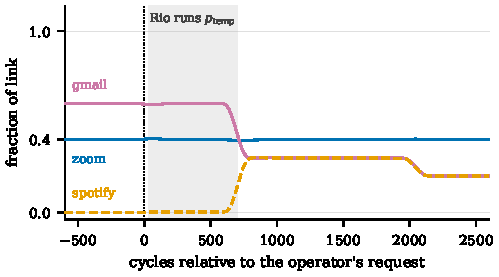
\includegraphics{fig-eval-ptemp.pdf}
\caption{The three flows under Rio's confined replace. The gray band is the interval in which Rio runs $p_\text{temp}$.}
\label{fig:eval-ptemp}
\end{figure}

The traffic is the traffic of \cref{sec:eval}.
\textsf{zoom} sends enough packets to fill 40\% of the link throughout, \textsf{gmail} fills 80\% before the request and 20\% after it, and \textsf{spotify} starts sending when the request arrives, enough to fill 20\%.

\Cref{fig:eval-ptemp} shows what each of the three flows receives.
\textsf{zoom} holds the high-priority arm but asks for only 0.40 of the link and gets it, so \textsf{gmail} takes the remainder.
\textsf{gmail} is lifted while \textsf{gmail}\textsubscript{old} drains ahead of new arrivals, and \textsf{spotify} waits on that drain, reaching first service 709 cycles after the request against the stop-the-world baseline's 1408.

\end{document}
